\vspace{15cm}
\chapter{Pengujian Model dan Skema} \label{bab uji}

\noindent Model dan skema pembelajaran mesin atau \emph{machine learning} (ML) yang telah dibahas pada Bab \ref{bab jsf} dan \ref{bab skema} akan diimplementasikan ke dalam program. Program ini akan dirancang sedemikian sehingga hasil rancangannya berbentuk GUI. Konstruksi programnya akan dijelaskan pada Subbab \ref{konst program}. Program ini dirancang untuk membangun model jaringan saraf fuzzy (JSF) dengan tiga skema klasifikasi multikelas. Program ini juga ditujukan untuk menguji model JSF yang telah diperoleh.

\noindent Data yang digunakan untuk membangun dan menguji model JSF telah memenuhi syarat-syarat yang disebutkan pada Bab \ref{bab satu}. Terdapat empat data yang digunakan. Empat data ini akan dijelaskan lebih lanjut pada Subbab \ref{tentang data}. Selanjutnya, akan dibahas hasil pengujian model JSF dan skema klasifikasi multikelas terhadap masing-masing dari empat data ini. Hasil dari pengujian terhadap data ini dibahas pada Subbab \ref{hasil uji}.

\section{Konstruksi Program} \label{konst program}
\noindent Tampilan awal dari program yang telah dirancang oleh penulis dapat dilihat pada \ref{fig: tampilan awal}. Untuk membangun model JSF menggunakan program ini, pengguna harus memasukkan data terlebih dahulu menggunakan tombol `\colorbox{gray!30}{Insert dataset}' (\ref{fig: ss 01}). Selanjutnya, pengguna diminta untuk menentukan fitur-fitur yang akan digunakan (\ref{fig: ss 02}).

\begin{figure}[htbp!]
\begin{subfigure}[h]{0.49\textwidth}
  \centering
  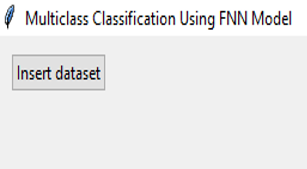
\includegraphics[width=\linewidth]{SSprogram/01Awal.png}  
  \caption{}
  \label{fig: ss 01}
\end{subfigure}
\begin{subfigure}[h]{0.49\textwidth}
  \centering
  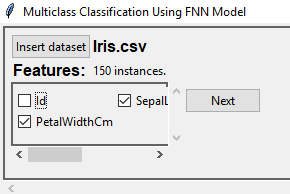
\includegraphics[width=.7\linewidth]{SSprogram/02-Select-features.png}
  \caption{}
  \label{fig: ss 02}
\end{subfigure}
\caption{Tampilan awal program}
\label{fig: tampilan awal}
\end{figure}

\noindent Program ini menyediakan beberapa pilihan untuk tahap pra pemrosesan data. Pada \ref{fig: ss 03}, kotak berwarna biru digunakan untuk menentukan fitur-fitur yang berupa kategori. Di samping itu, pengguna memiliki pilihan terkait data uji yang digunakan. Pilihan ini disediakan pada kotak merah (\ref{fig: ss 03}). Jika data uji yang digunakan terpisah dari data yang telah dimasukkan, maka nantinya pengguna harus memasukkan data uji. Jika data uji ingin dipisahkan menggunakan program ini yang dibantu oleh \emph{package sklearn} python, maka pengguna harus memasukkan ukuran data uji dan \emph{random state} seperti pada kotak biru di dalam \ref{fig: ss 04}. Untuk setiap data, dua nilai yang ada di kotak biru ini dibuat tetap sebagaimana yang tercantum di dalam gambar.

\begin{figure}[h!]
\begin{subfigure}[h]{\textwidth}
  \centering
  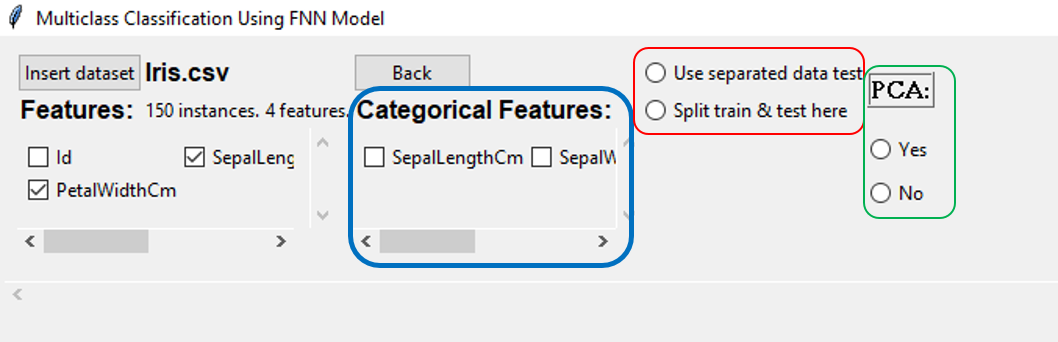
\includegraphics[width=.98\linewidth]{SSprogram/03.png}  
  \caption{}
  \label{fig: ss 03}
\end{subfigure}
\\
\begin{subfigure}[h]{\textwidth}
  \centering
  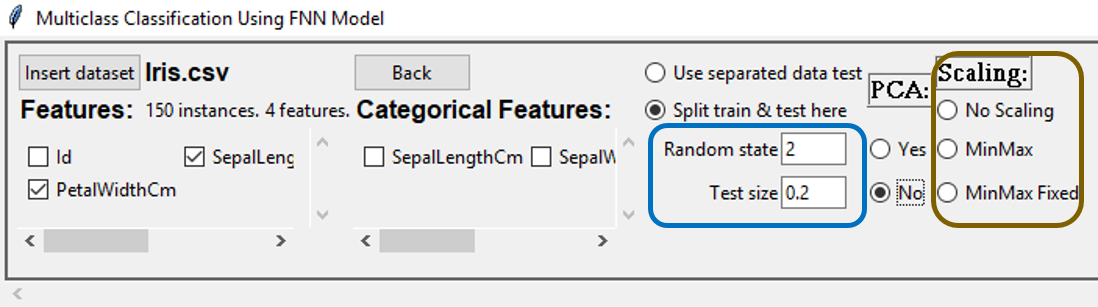
\includegraphics[width=.98\linewidth]{SSprogram/04.png}
  \caption{}
  \label{fig: ss 04}
\end{subfigure}%
\\
\begin{subfigure}[h]{\textwidth}
  \centering
  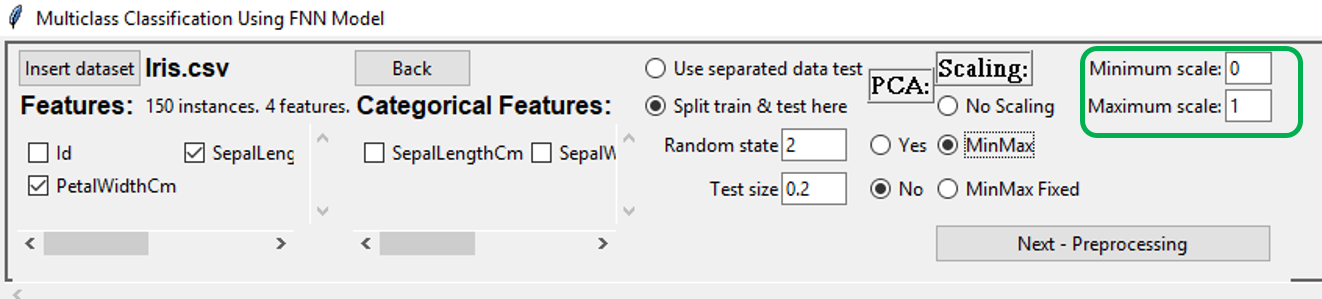
\includegraphics[width=.98\linewidth]{SSprogram/05.png}  
  \caption{}
  \label{fig: ss 05}
\end{subfigure}
\caption{Pilihan yang disediakan oleh program pada tahap pra pemrosesan data}
\label{fig: pra pemrosesan}
\end{figure}

\noindent Pilihan untuk menggunakan PCA atau tidak menggunakannya juga disediakan oleh program ini. Jika ingin menggunakan PCA, maka program secara otomatis akan menggunakan normalisasi standar untuk penskalaan dan pengguna akan diminta untuk memasukkan banyaknya komponen utama yang diinginkan. Jika tidak, maka pengguna akan memilih jenis penskalaan nilai pada data latih sesuai dengan yang tertera di dalam kotak berwarna emas pada \ref{fig: ss 04}. Pilihan `\emph{MinMax Fixed}' digunakan ketika fitur-fitur pada data memiliki skala nilai yang sama, diketahui nilai minimum dan maksimumnya, serta nilai-nilai dari fitur berpeluang tidak dapat diterima oleh model JSF. Pilihan `\emph{MinMax Fixed}' dan `\emph{MinMax}' sama-sama akan meminta nilai skala minimal dan maksimal yang diinginkan (\ref{fig: ss 05}). Selanjutnya, dengan menekan tombol `\colorbox{gray!30}{Next - Preprocessing}', maka program akan melakukan pra pemrosesan data sesuai dengan pilihan pengguna yang telah dibahas sebelumnya.

\begin{figure}[h!]
\begin{subfigure}[h]{\textwidth}
  \centering
  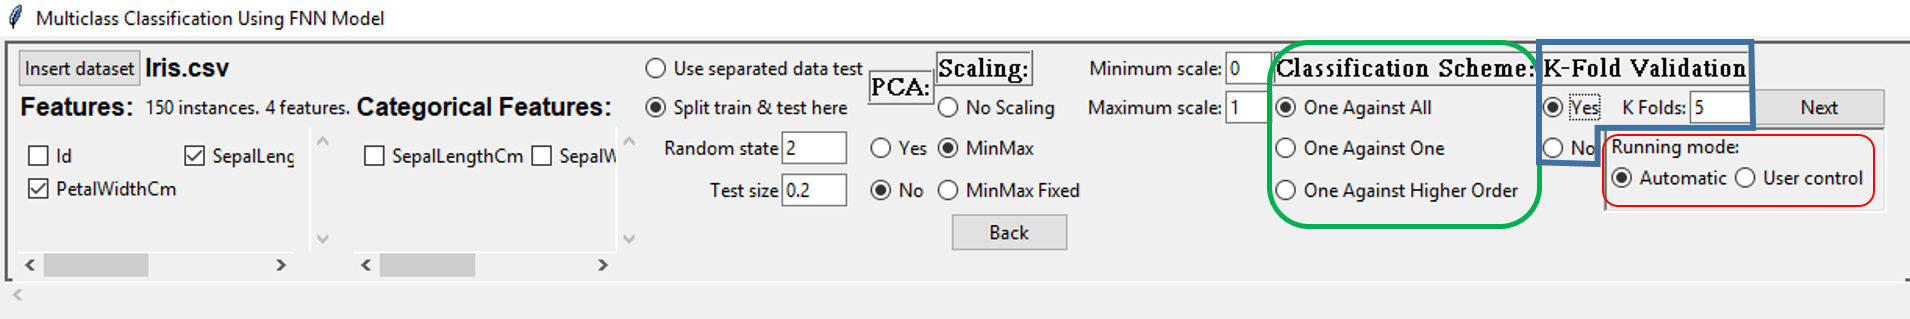
\includegraphics[width=.98\linewidth]{SSprogram/06.png}  
  \caption{}
  \label{fig: ss 06}
\end{subfigure}
\\
\begin{subfigure}[h]{\textwidth}
  \centering
  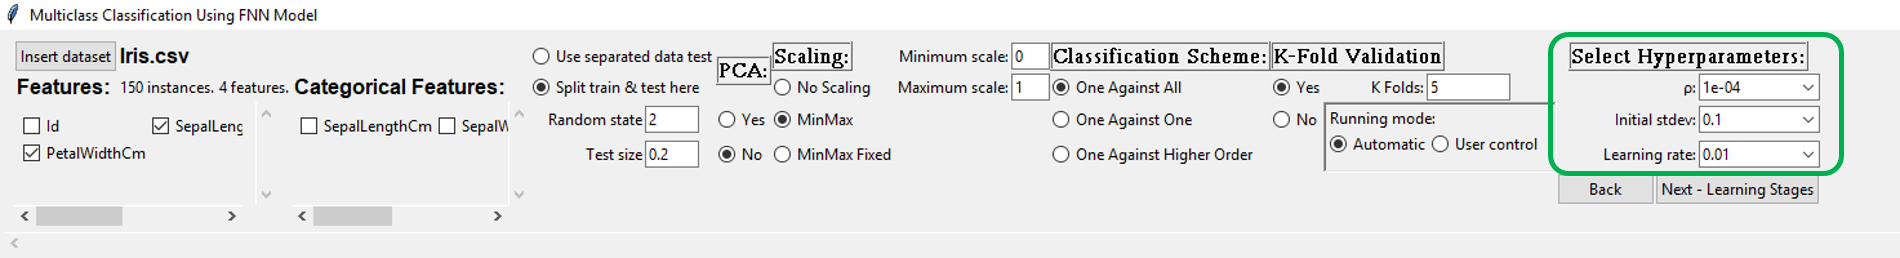
\includegraphics[width=.98\linewidth]{SSprogram/07.png}
  \caption{}
  \label{fig: ss 07}
\end{subfigure}%
\\
\begin{subfigure}[h]{\textwidth}
  \centering
  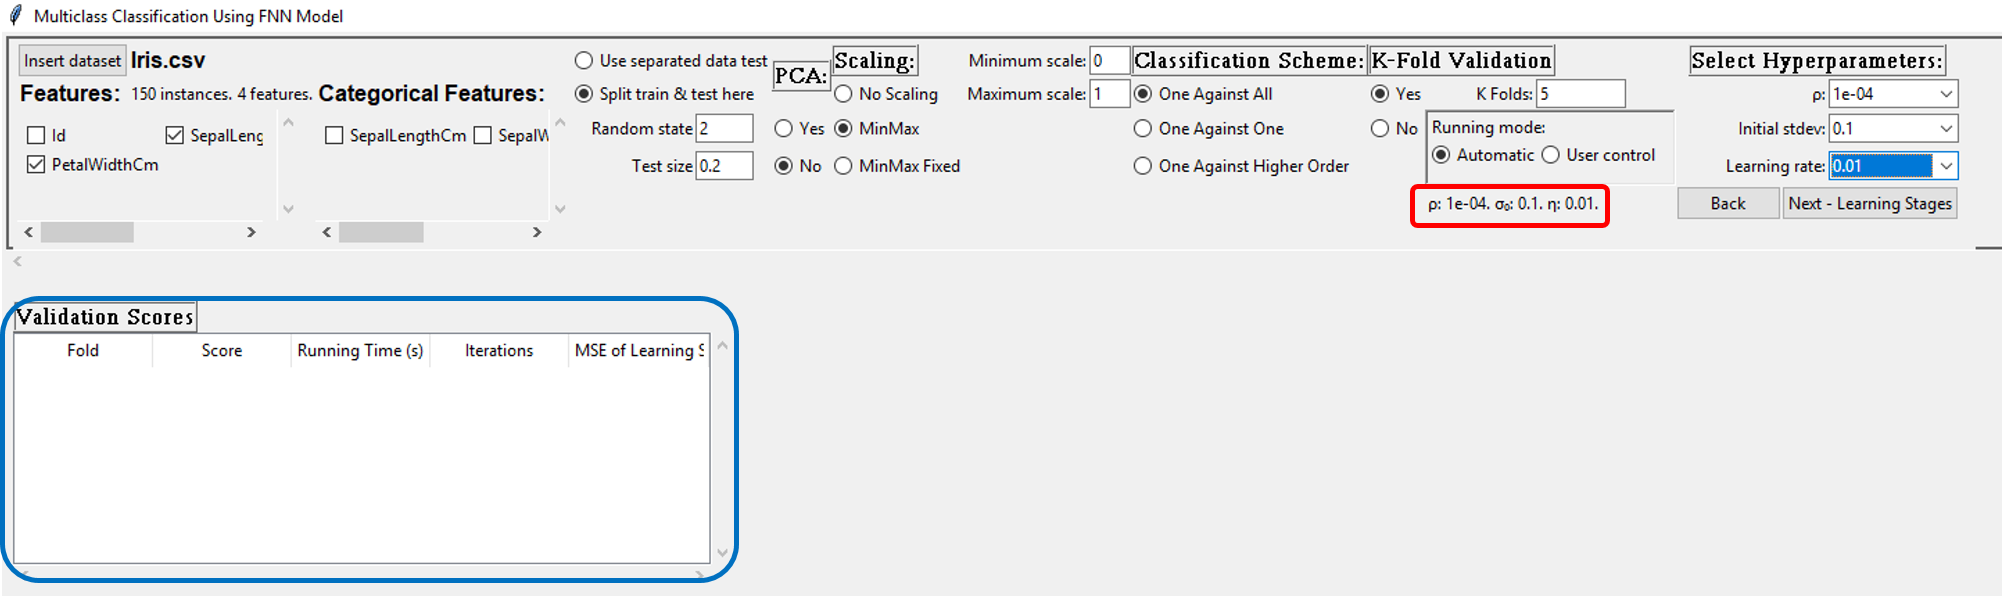
\includegraphics[width=.98\linewidth]{SSprogram/08.png}  
  \caption{}
  \label{fig: ss 08}
\end{subfigure}
\caption{Pemilihan skema klasifikasi multikelas, validasi silang, dan hiperparameter}
\label{fig: skema klas, cv, dan hyperpar}
\end{figure}

\noindent \ref{fig: skema klas, cv, dan hyperpar} menunujukkan bahwa program ini dapat menyediakan berbagai pilihan untuk menentukan skema ML. Di dalam kotak hijau pada \ref{fig: ss 06} pengguna dapat memilih skema klasifikasi multikelas yang akan digunakan. Pilihan \emph{running mode} di dalam kotak merah pada \ref{fig: ss 06} menyediakan pilihan mode untuk menjalankan skema pembangunan model JSF. Jika pengguna ingin menentukan nilai dari batas galat dan iterasi maksimal secara manual, serta ingin melanjutkan \emph{running} ke sub data latih berikutnya dengan cara manual, maka gunakan pilihan `\emph{user control}'. Jika pengguna menginginkan program secara otomatis dapat membangun dan menguji model JSF dari awal sampai dengan selesai, maka gunakan pilihan `\emph{automatic}'. Ketika memilih pilihan ini, maka nilai dari batas galat dan iterasi maksimal, berturut-turut, ditetapkan sebesar $10^{-4}$ dan 1.000. Sebagian besar data dan skema klasifikasi multikelas menggunakan pilihan `\emph{automatic}' untuk membangun model JSF berdasarkan data tersebut.

\noindent Pilihan antara akan menggunakan validasi silang atau tidak menggunakannya terdapat di dalam kotak biru pada \ref{fig: ss 06}. Lebih jauh lagi, jika pengguna memilih untuk menggunakan validasi silang, program ini akan menyediakan fasilitas berupa banyaknya \emph{fold} (sub data latih) yang diinginkan. Pada skema pembangunan model JSF dan pengujian setiap data di dalam tugas akhir ini, pilihan ``tidak menggunakan validasi silang'' digunakan ketika hiperparameter `terbaik' telah diperoleh untuk suatu skema klasifikasi multikelas.

\noindent Bagian yang cukup penting dalam skema pembangunan model ML, termasuk model JSF, adalah penentuan nilai dari hiperparameter. Penentuan nilai-nilai hiperparameter disediakan di dalam kotak hijau pada \ref{fig: ss 07}. Pada tugas akhir ini, hiperparameter yang akan berubah-ubah adalah $\rho$, $s_0$, dan $\eta$. Nilai $\tau$ dijadikan tetap.

\noindent Berikut ini adalah penjelasan mengenai alasan dari nilai $\tau$ yang dijadikan tetap. Berdasarkan penjelasan pada Subbab \ref{skema klasifikasi}, setiap skema klasifikasi multikelas mengakibatkan model JSF hanya bernilai 0 atau 1 pada semua neuron di dalam lapisan keluaran. Dalam skema OAA, nilai neuron-neuron pada lapisan keluaran dari observasi ke-$l$ dinyatakan dengan $\mathbf{d}^{(l)} = (d^{(l)}_1, d^{(l)}_2, \ldots, d^{(l)}_p)$ dengan $p$ menyatakan banyaknya label kelas yang berbeda pada data. Pada skema OAA, jika observasi ke-$l$ memiliki label kelas $\mathcal{C}_k$, maka entri ke-$k$ dari vektor $\mathbf{d}^{(l)}$ bernilai 1 dan entri yang tersisa bernilai 0. Akibatnya, nilai dari $u$ pada (\ref{kriteria kemiripan keluaran}) selalu sama dengan $\sqrt{2}$. Dalam skema OAO dan OAHO, nilai neuron pada lapisan keluaran dari setiap jaringannya hanya di antara 0 atau 1. Akibatnya, nilai dari $u$ pada (\ref{kriteria kemiripan keluaran}) selalu sama dengan $1$. Dengan demikian, untuk setiap $\tau<1$ pada Pertidaksamaan (\ref{kriteria kemiripan keluaran}) akan menghasilkan keputusan yang sama terkait kemiripan data keluaran dengan klaster yang telah terbentuk dalam fase identifikasi struktur. Jadi, nilai hiperparameter $\tau$ dapat dijadikan tetap. Pada model JSF yang dibangun melalui tugas akhir ini, ditetapkan $\tau = \num{0,3}$.

\noindent Nilai hiperparameter $\rho$ dipilih dari himpunan $\{ 10^{-4}\text{, } \allowbreak 10^{-8} \text{, } \allowbreak 10^{-12} \text{, } \allowbreak 10^{-20} \text{, } \allowbreak 10^{-25} \text{, } \allowbreak 10^{-50} \text{, } \allowbreak 10^{-75} \text{, } \allowbreak 10^{-125} \text{, } \allowbreak 10^{-200} \text{, } \allowbreak 10^{-275} \text{, } \allowbreak 10^{-350} \}$. Nilai $\rho$ yang sangat kecil digunakan ketika data berdimensi cukup besar atau nilai simpangan baku dari fitur-fiturnya cukup besar. Nilai hiperparameter $s_0$ dipilih dari himpunan $\{\num{0,1} \text{, } \allowbreak \num{0,2} \text{, } \allowbreak \num{0,25} \text{, } \allowbreak \num{0,3} \text{, } \allowbreak \num{0,4} \text{, } \num{0,5} \text{, } \allowbreak \num{0,6}\}$ yang setiap anggotanya dikalikan dengan selisih antara nilai miksimum dan minimum dari keseluruhan nilai fitur. Nilai hiperparameter $\eta$ dipilih dari himpunan $\{\num{0,01} \text{, } \allowbreak \num{0,05} \text{, } \allowbreak \num{0,1}\}$.

\noindent Setelah setiap hiperparameter dipilih, maka program akan menampilkan nilai-nilai hiperparameter yang akan digunakan, sebagaimana tertera di dalam kotak merah pada \ref{fig: ss 08}. Selain itu, akan ditampilkan juga tabel skor akurasi untuk validasi silang pada kotak biru. Tabel ini akan terisi ketika satu iterasi dari proses validasi silang telah selesai. Selanjutnya, gunakan tombol `\colorbox{gray!30}{Next - Learning Stages}' untuk memasuki tahap utama dari pembelajaran mesin ini.

\begin{figure}[h!]
\begin{subfigure}[h]{\textwidth}
  \centering
  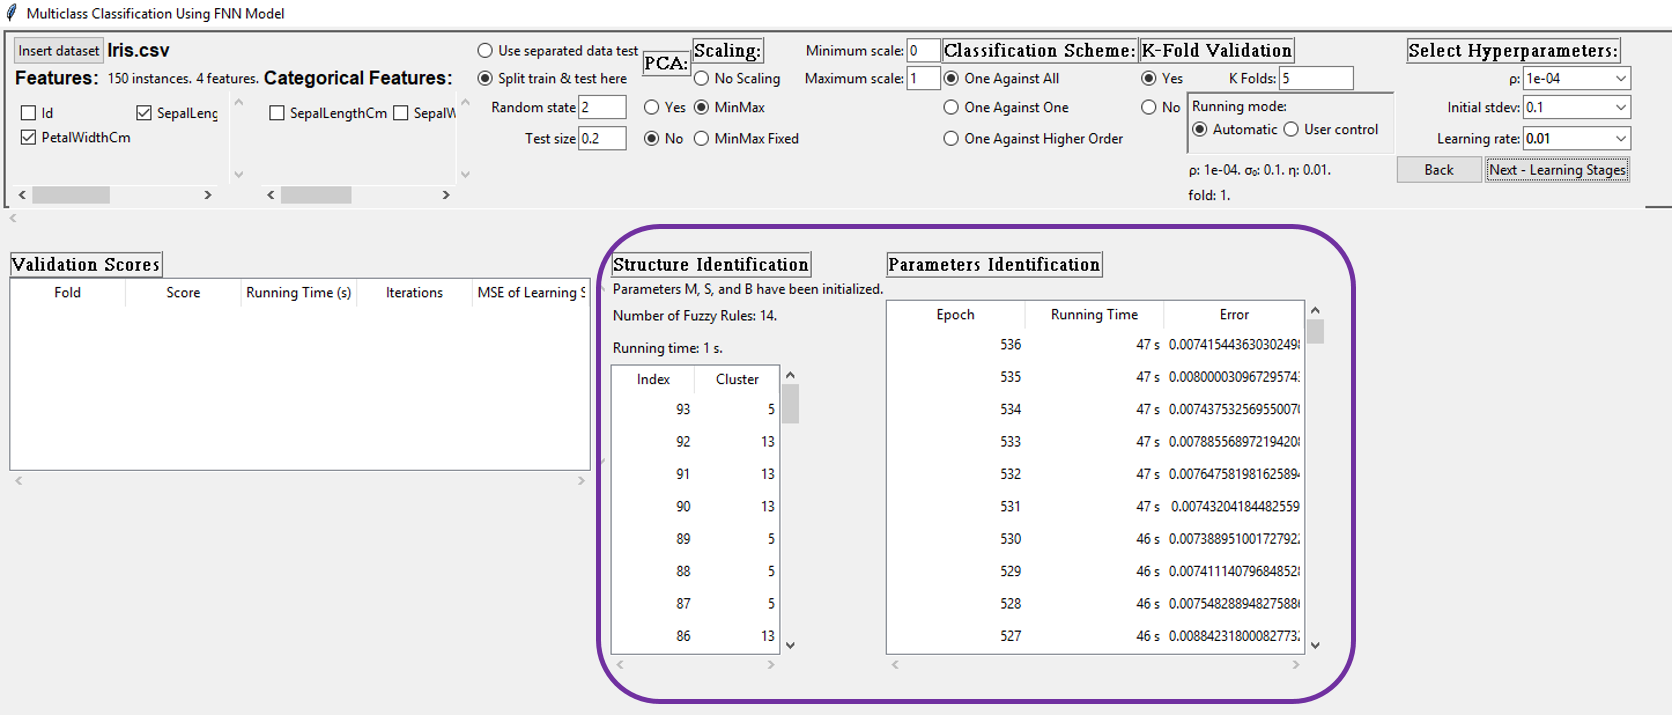
\includegraphics[width=.93\linewidth]{SSprogram/09.png}  
  \caption{Skema OAA}
  \label{fig: ss 09}
\end{subfigure}
\\
\begin{subfigure}[h]{0.5\textwidth}
  \centering
  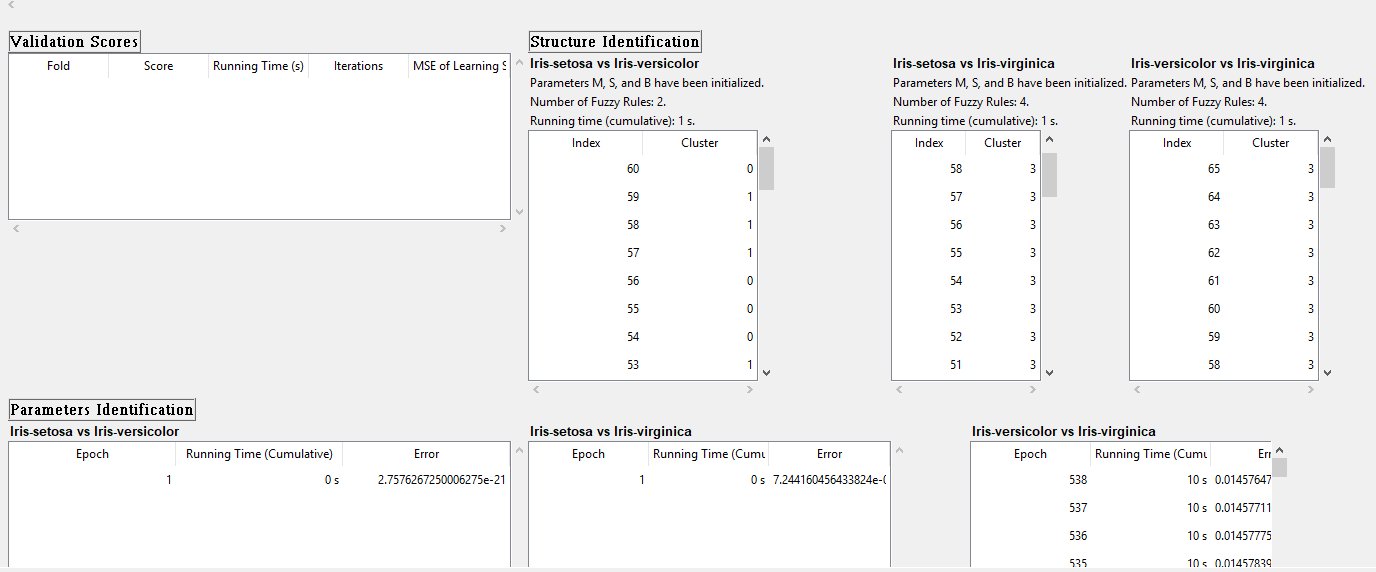
\includegraphics[width=.98\linewidth]{SSprogram/09b.png}
  \caption{Skema OAO}
  \label{fig: ss 09b}
\end{subfigure}%
\begin{subfigure}[h]{0.5\textwidth}
  \centering
  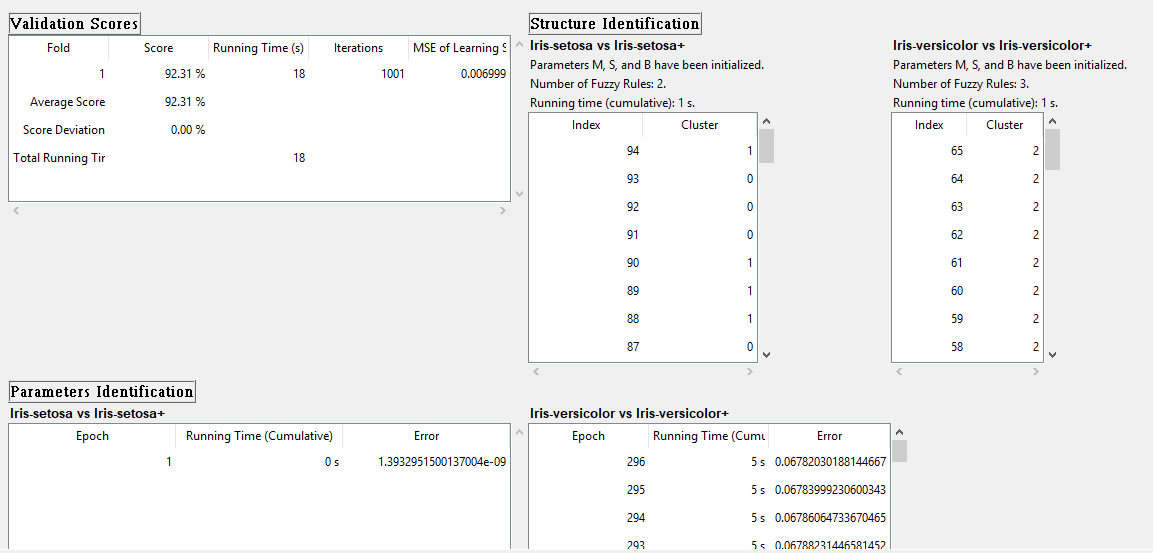
\includegraphics[width=.93\linewidth]{SSprogram/09c.png}  
  \caption{Skema OAHO}
  \label{fig: ss 09c}
\end{subfigure}
\caption{Proses pembangunan dan pengujian model jaringan saraf fuzzy}
\label{fig: proses pembelajaran dan pengujian}
\end{figure}

\noindent Proses pembangunan model ditampilkan seperti pada \ref{fig: proses pembelajaran dan pengujian}. Pada gambar tersebut ditampilkan contoh proses pembangunan model JSF dengan skema yang berbeda. Setiap skema klasifikasi multikelas memiliki tampilan yang berbeda-beda karena banyaknya jaringan yang terbentuk juga berbeda. Dalam kotak berwarna ungu pada \ref{fig: ss 09}, skema OAA hanya melakukan satu kali fase identifikasi struktur dan identifikasi parameter. Ini dikarenakan skema OAA hanya membentuk satu jaringan dari model JSF. Sebagaimana telah dijelaskan pada Subbab \ref{skema klasifikasi} bahwa skema OAO dan OAHO menghasilkan model JSF dengan jaringan berganda. Akibatnya, skema OAO dan OAHO (\ref{fig: ss 09b} dan \ref{fig: ss 09c}) melakukan lebih dari satu kali identifikasi struktur dan identifikasi parameter.

\begin{figure}[h!]
\begin{subfigure}[h]{\textwidth}
  \centering
  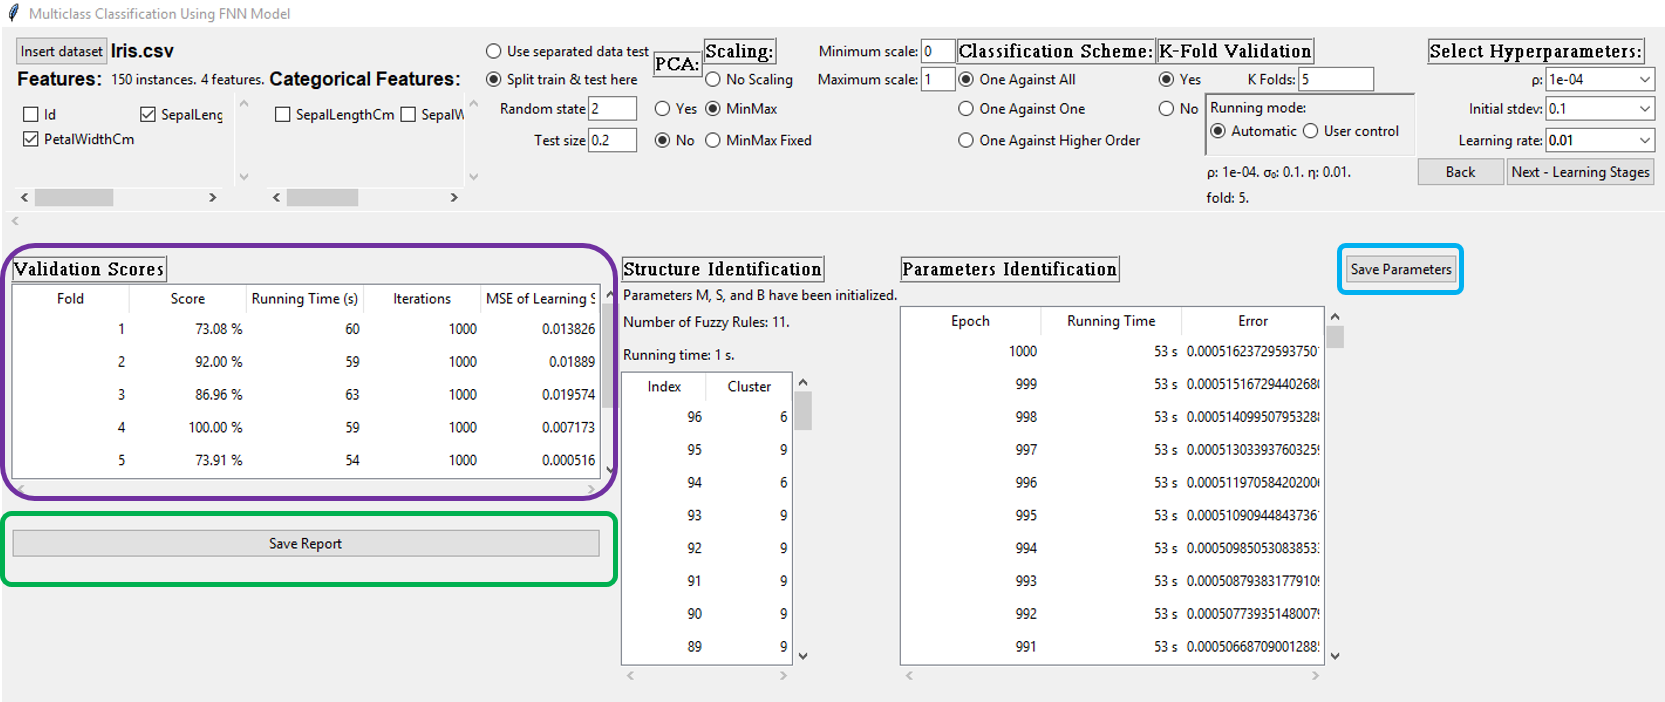
\includegraphics[width=.98\linewidth]{SSprogram/10.png}  
  \caption{}
  \label{fig: ss 10}
\end{subfigure}
\\
\begin{subfigure}[h]{\textwidth}
  \centering
  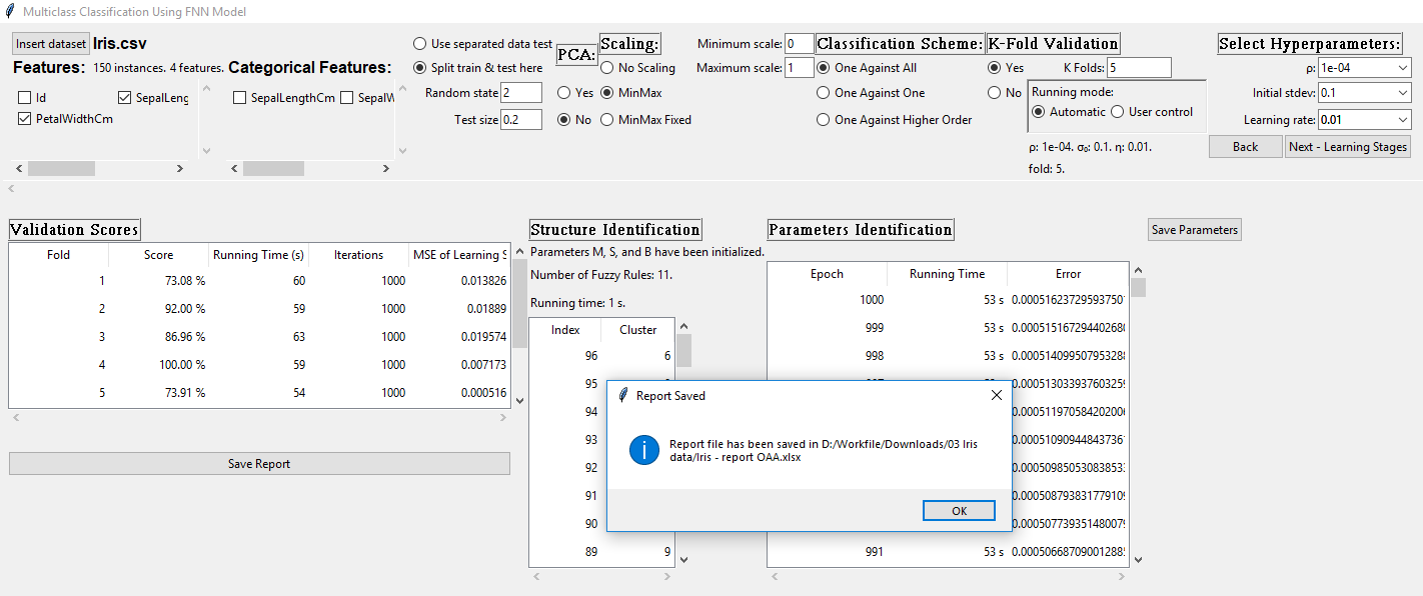
\includegraphics[width=.98\linewidth]{SSprogram/11.png}
  \caption{}
  \label{fig: ss 11}
\end{subfigure}%
\caption{Proses penyimpanan hasil uji}
\label{fig: proses penyimpanan hasil uji}
\end{figure}

\noindent Jika satu kali validasi silang telah diproses, maka akan ditampilkan skor akurasi dari data validasi seperti yang tertera di dalam kotak ungu pada \ref{fig: ss 10}. Setelah semua validasi silang selesai, maka pengguna dapat menekan tombol `\colorbox{gray!30}{Save Report}' (yang ada di dalam kotak berwarna hijau) untuk menyimpan skor akurasi dari setiap data validasi berdasarkan hiperparameter tertentu ke dalam \emph{Ms. Excel}. \ref{fig: ss 11} menunjukkan bahwa proses penyimpanan file yang diinginkan berjalan dengan lancar. Selain itu, juga diperlihatkan lokasi dan nama file yang telah disimpan. Tombol `\colorbox{gray!30}{Save Parameters}' di dalam lingkaran biru pada \ref{fig: ss 10} berfungsi untuk menyimpan nilai-nilai dari parameter yang diperoleh, yaitu matriks $\mathbf{M}$, $\mathbf{S}$, dan kumpulan matriks $\mathbf{B}_i$ ke dalam \emph{Ms. Excel}.

\noindent Proses validasi silang tersebut dilakukan berulang-ulang menggunakan nilai hiperparameter yang berbeda. Setelah model JSF memiliki skor akurasi yang optimal, maka hiperparameter yang terlibat dalam skema pembangunan model JSF tersebut digunakan untuk mendapatkan model JSF berdasarkan data latih secara keseluruhan, bukan dari beberapa sub data latih. Setelah itu, model yang diperoleh akan diuji terhadap data uji untuk mendapatkan skor akurasi model pada data uji.

\section{Deskripsi dan Analisis Data} \label{tentang data}
\noindent Data yang digunakan di antaranya adalah data koordinat I, data koordinat II, data tanaman iris, dan data evaluasi mobil. Dua data pertama dibangkitkan menggunakan bahasa pemrograman python. Dua data terakhir diambil dari situs web UCI \emph{Machine Learning Repository}. Tiga data pertama merupakan data yang seimbang. Hal ini dikarenakan setiap tiga data tersebut memiliki kardinalitas yang sama untuk setiap label kelasnya. Selain itu, nilai dari fitur-fitur pada tiga data pertama berupa bilangan real. Nilai dari fitur-fitur pada data terakhir berupa kategori. Data-data tersebut belum dipisahkan menjadi data latih dan data uji. Oleh karena itu, untuk setiap data akan dipisahkan menjadi data latih dan data uji pada tahap pra pemrosesan data.

\noindent Sebelum setiap data digunakan untuk membangun dan menguji model dan skema JSF, akan dilakukan analisis terhadap masing-masing data terlebih dahulu.Pada analisis data ini, dari masing-masing data akan dicari rata-rata, simpangan baku, median, nilai minimal, dan nilai maksimal untuk setiap fitur yang berupa bilangan real. Untuk fitur yang berupa kategori, akan dicari kardinalitas setiap kategorinya.

\subsection{Data Koordinat I} \label{tentang dk1}
\noindent Data koordinat I terdiri dari 1.000 observasi. Setiap observasi mempunyai tiga fitur yang masing-masing menjelaskan koordinat observasi tersebut pada sumbu $x$, $y$, dan $z$. Nilai-nilai untuk setiap fitur pada setiap observasi hanya berupa bilangan bulat. Label pada data koordinat I berupa nomor oktan. Banyaknya nomor oktan yang berbeda ada 8. Dengan demikian, data ini terdiri dari 8 label kelas.

\noindent Data ini terdiri dari tiga fitur. Akibatnya, setiap observasi yang ada di dalam data ini merupakan rangkap tiga terurut dari bilangan bulat. Pada data koordinat I, rangkap tiga terurut ini dibangkitkan dengan cara menentukan permutasi tiga angka yang diambil dari himpunan $U_1 = \{-5\leq u \leq -1 \text{ atau } 1 \leq u \leq 5 : u \in \mathbb{Z} \}$. Banyaknya permutasi yang mungkin adalah 1.000. Dengan demikian, semua permutasi termuat di dalam data koordinat I. Selanjutnya, setiap observasi diberi label berupa nomor oktan berdasarkan tanda pada masing-masing fiturnya. Karena semua permutasi termuat di dalam data, maka kardinalitas untuk masing-masing label kelas pada data ini adalah sama, yaitu 125. Data koordinat I dilampirkan pada Lampiran \ref{lam: data koord I}. Berikut ini hanya ditampilkan statistika deskriptifnya saja.

\begin{table}[htbp!]
  \centering
  \caption{Statistika deskriptif untuk setiap fitur dari data koordinat I}
    \begin{tabular}{lrrr}
    \toprule
    \multicolumn{1}{c}{\multirow{2}[4]{*}{\textbf{Statistika deskriptif}}} & \multicolumn{3}{c}{\textbf{Fitur}} \\
\cmidrule{2-4}          & \multicolumn{1}{c}{\boldmath{}$x$\unboldmath{}} & \multicolumn{1}{c}{\boldmath{}$y$\unboldmath{}} & \multicolumn{1}{c}{\boldmath{}$z$\unboldmath{}} \\
\cmidrule{2-4}    \textbf{Median} & $\num{0}$ & $\num{0}$ & $\num{0}$ \\
    \textbf{Rata-rata} & $\num{0}$ & $\num{0}$ & $\num{0}$ \\
    \textbf{Simpangan baku} & $\num{3,318}$ & $\num{3,318}$ & $\num{3,318}$ \\
    \textbf{Minimum} & $\num{-5}$ & $\num{-5}$ & $\num{-5}$ \\
    \textbf{Maksimum} & $\num{5}$ & $\num{5}$ & $\num{5}$ \\
    \bottomrule
    \end{tabular}%
  \label{tab: stat desc dk1}%
\end{table}%

\subsection{Data Koordinat II} \label{tentang dk2}
\noindent Berikut ini adalah statistika deskriptif untuk masing-masing fitur dari data koordinat II.

\begin{table}[htbp!]
  \centering
  \caption{Statistika deskriptif untuk setiap fitur dari data koordinat II}
    \begin{tabular}{lrrr}
    \toprule
    \multicolumn{1}{c}{\multirow{2}[4]{*}{\textbf{Statistika deskriptif}}} & \multicolumn{3}{c}{\textbf{Fitur}} \\
\cmidrule{2-4}          & \multicolumn{1}{c}{\boldmath{}$x$\unboldmath{}} & \multicolumn{1}{c}{\boldmath{}$y$\unboldmath{}} & \multicolumn{1}{c}{\boldmath{}$z$\unboldmath{}} \\
\cmidrule{2-4}    \textbf{Median} & $\num{0}$ & $\num{0}$ & $\num{0}$ \\
    \textbf{Rata-rata} & $\num{-0,091}$ & $\num{0,255}$ & $\num{0,022}$ \\
    \textbf{Simpangan baku} & $\num{56,61}$ & $\num{58,32}$ & $\num{59,04}$ \\
    \textbf{Minimum} & $\num{-100}$ & $\num{-100}$ & $\num{-100}$ \\
    \textbf{Maksimum} & $\num{100}$ & $\num{100}$ & $\num{100}$ \\
    \bottomrule
    \end{tabular}%
  \label{tab: stat desc dk2}%
\end{table}%

\noindent Data koordinat II mirip dengan data koordinat I. Perbedaannya terletak pada bilangan bulat rangkap tiga terurut yang dibangkitkan. Pada data koordinat II, rangkap tiga terurut adalah sebanyak 1.000 permutasi tiga angka dari himpunan $U_2 = \{-100\leq u \leq -1 \text{ atau } 1 \leq u \leq 100 : u \in \mathbb{Z} \}$. Banyaknya permutasi adalah $200^3 = 8\times 10^6$. Dengan demikian, hanya $\num{0,0125}\%$ dari semua kemuangkinan permutasi  yang termuat di dalam data koordinat II. Kardinalitas untuk masing-masing label kelas pada data ini dibuat sama, yaitu 125. Data ini dilampirkan pada Lampiran \ref{lam: data koord II}.

\subsection{Data Tanaman Iris} \label{tentang d iris}
\noindent Data ini memuat 3 kelas yang masing-masing terdiri dari 50 observasi. Setiap kelas mengacu pada jenis tanaman iris, yaitu: iris \emph{setosa}, iris \emph{versicolor}, dan iris \emph{virginica}. Setiap observasi memiliki 4 fitur, yaitu: panjang sepal (cm), lebar sepal (cm), panjang kelopak (cm), dan lebar kelopak (cm). Data tanaman iris merupakan data yang paling dikenal dan paling sering ditemukan dalam literatur pengenalan pola yang termasuk ke dalam masalah klasifikasi multikelas \cite{Dua:2019}. Data ini dilampirkan pada Lampiran \ref{lam: data iris}. Berikut ini hanya ditampilkan statistika deskriptifnya saja.

\begin{table}[htbp!]
  \centering
  \caption{Statistika deskriptif untuk setiap fitur dari data tanaman iris}
    \begin{tabular}{lrrrr}
    \toprule
    \multicolumn{1}{c}{\multirow{2}[3]{*}{\textbf{Statistika deskriptif}}} & \multicolumn{4}{c}{\textbf{Fitur}} \\
\cmidrule{2-5}    \multicolumn{1}{c}{} & \multicolumn{1}{>{\centering\arraybackslash} m{3.515em}}{\textbf{Panjang sepal}} & \multicolumn{1}{>{\centering\arraybackslash} m{3.115em}}{\textbf{Lebar sepal}} & \multicolumn{1}{>{\centering\arraybackslash} m{3.515em}}{\textbf{Panjang kelopak}} & \multicolumn{1}{>{\centering\arraybackslash} m{3.515em}}{\textbf{Lebar kelopak}} \\
    \cmidrule{2-5}
    \textbf{Median} & $\num{5,8}$ & $\num{3}$ & $\num{4,35}$ & $\num{1,3}$ \\
    \textbf{Rata-rata} & $\num{5,843}$ & $\num{3,054}$ & $\num{3,759}$ & $\num{1,199}$ \\
    \textbf{Simpangan baku} & $\num{0,8281}$ & $\num{0,4336}$ & $\num{1,764}$ & $\num{0,7632}$ \\
    \textbf{Minimum} & $\num{4,3}$ & $\num{2}$ & $\num{1}$ & $\num{0,1}$ \\
    \textbf{Maksimum} & $\num{7,9}$ & $\num{4,4}$ & $\num{6,9}$ & $\num{2,5}$ \\
    \bottomrule
    \end{tabular}%
  \label{tab: stat desc iris}%
\end{table}%

\noindent 

\subsection{Data Evaluasi Mobil} \label{tentang car}
\noindent Data evaluasi mobil menceritakan spesifikasi dan klasifikasi dari 1.728 mobil. Setiap mobil pada data ini diklasifikasikan ke dalam 4 label kelas berdasarkan kualitasnya. Empat label kelas ini adalah kualitas mobil yang \emph{unaccepted}, \emph{accepted}, \emph{good}, dan \emph{very good}. Setiap label kelas memiliki banyaknya observasi yang berbeda-beda. Banyaknya mobil dengan kualitas yang \emph{unaccepted},  \emph{accepted}, \emph{good}, dan \emph{very good} berturut-turut adalah 1210, 384, 69, dan 65. Setiap mobil yang ada di dalam data ini dideskripsikan oleh 6 kategori spesifikasi, yaitu:
\begin{itemize}
    \item \emph{Buying}, yaitu kategori harga beli mobil yang meliputi \emph{very high}, \emph{high}, \emph{medium}, dan \emph{low},
    \item \emph{Maintenance}, yaitu biaya pemeliharaan mobil yang kategorinya sama dengan kategori pada spesifikasi \emph{buying},
    \item \emph{Doors}, yaitu kategori banyaknya pintu mobil, terdiri dari 4 kategori yang berbeda: dua pintu, tiga pintu, empat pintu, dan kategori lima pintu atau lebih,
    \item \emph{Persons}, yaitu kategori banyaknya maksimal orang yang berada di dalam mobil, meliputi: kategori dua orang, kategori empat orang, dan kategori lebih dari empat orangm,
    \item \emph{Lug boot}, yaitu kategori ukuran bagasi mobil yang meliputi ukuran kecil, sedang, dan besar,
    \item \emph{Safety}, yaitu tingkat keamanan bagi pengendara dan penumpang, meliputi tingkat keamanan rendah, sedang, dan tinggi.
\end{itemize}

\begin{table}[htbp!]
  \centering
  \caption{Kardinalitas setiap kategori pada setiap fitur dari data evaluasi mobil}
    \begin{tabular}{crcrcr}
    \toprule
    \multicolumn{2}{c}{\textit{\textbf{Buying}}} & \multicolumn{2}{c}{\textit{\textbf{Maintenance}}} & \multicolumn{2}{c}{\textit{\textbf{Doors}}} \\
    \cmidrule(r){1-2}\cmidrule(lr){3-4}\cmidrule(l){5-6}
    \textbf{Kategori} & \multicolumn{1}{c}{\textbf{Kardinalitas}} & \textbf{Kategori} & \multicolumn{1}{c}{\textbf{Kardinalitas}} & \textbf{Kategori} & \multicolumn{1}{c}{\textbf{Kardinalitas}} \\
    \cmidrule(r){1-2}\cmidrule(lr){3-4}\cmidrule(l){5-6}
    \textit{\textbf{med}} & 432   & \textit{\textbf{med}} & 432   & \textit{\textbf{two}} & 432 \\
    \textit{\textbf{high}} & 432   & \textit{\textbf{high}} & 432   & \textit{\textbf{four}} & 432 \\
    \textit{\textbf{low}} & 432   & \textit{\textbf{low}} & 432   & \textit{\textbf{three}} & 432 \\
    \textit{\textbf{vhigh}} & 432   & \textit{\textbf{vhigh}} & 432   & \textit{\textbf{5more}} & 432 \\
    \midrule
          &       &       &       &       &  \\
    \midrule
    \multicolumn{2}{c}{\textit{\textbf{Persons}}} & \multicolumn{2}{c}{\textit{\textbf{Lug boot}}} & \multicolumn{2}{c}{\textit{\textbf{Safety}}} \\
    \cmidrule(r){1-2}\cmidrule(lr){3-4}\cmidrule(l){5-6}
    \textbf{Kategori} & \multicolumn{1}{c}{\textbf{Kardinalitas}} & \textbf{Kategori} & \multicolumn{1}{c}{\textbf{Kardinalitas}} & \textbf{Kategori} & \multicolumn{1}{c|}{\textbf{Kardinalitas}} \\
    \cmidrule(r){1-2}\cmidrule(lr){3-4}\cmidrule(l){5-6}
    \textit{\textbf{two}} & 576   & \textit{\textbf{big}} & 576   & \textit{\textbf{med}} & 576 \\
    \textit{\textbf{four}} & 576   & \textit{\textbf{med}} & 576   & \textit{\textbf{high}} & 576 \\
    \textit{\textbf{more}} & 576   & \textit{\textbf{small}} & 576   & \textit{\textbf{low}} & 576 \\
    \bottomrule
    \end{tabular}%
  \label{tab: kard kat ev mobil}%
\end{table}%

\noindent Berdasarkan \ref{tab: kard kat ev mobil}, data evaluasi mobil memiliki kardinalitas yang seimbang antara setiap kategori pada masing-masing fiturnya. Karena semua fitur pada data ini berupa kategori, maka harus dilakukan pengkodean terlebih dahulu untuk setiap fiturnya. Pada tugas akhir ini, hanya akan dilakukan pengkodean dengan metode \emph{one hot encoding} yang telah dijelaskan pada Subbab \ref{preproccessing}. Setelah dilakukan \emph{one hot encoding}, banyaknya fitur pada data evaluasi mobil menjadi 21 dengan setiap entrinya berupa bilangan biner 0 atau 1. Data lengkap untuk data evaluasi mobil ini dilampirkan pada Lampiran \ref{lam: data mobil}.

\section{Hasil Uji} \label{hasil uji}
\noindent Pada tugas akhir ini, setiap data akan digunakan untuk membangun model JSF dengan skema tertentu dari klasifikasi multikelas. Tiga skema klasifikasi multikelas yang telah dijelaskan pada Subbab \ref{skema klasifikasi} akan digunakan untuk masing-masing data. Dengan demikian, terdapat 12 model JSF karena setiap data menghasilkan 3 model JSF dengan skema klasifikasi multikelas yang berbeda-beda.

\noindent Untuk setiap data dan skema klasifikasi, dilakukan validasi silang $K$-\emph{fold} untuk mendapatkan hiperparameter terbaik. Pada tugas akhir ini, hanya akan digunakan $K=5$, sehingga data latih dipartisi menjadi 5 sub data latih. Selanjutnya, dari 5 sub data latih ini akan diperoleh 5 \emph{learning set} dan 5 data validasi yang saling bersesuaian. Metode pembuatan 5 \emph{learning set} dan 5 data validasi ini telah dijelaskan pada Subbab \ref{pemilihan model}.

\noindent Pada validasi silang $5$-\emph{fold}, setiap \emph{learning set} akan digunakan untuk membangun model JSF dengan skema klasifikasi tertentu. Setiap model JSF yang diperoleh ini akan diuji pada data validasi. Hasil uji ini akan menghasilkan skor akurasi dari prediksi label kelas pada setiap observasi di dalam data validasi.  Dengan demikian, akan ada 5 model JSF dan 5 skor akurasi yang diperoleh. Untuk meringkas performa dari 5 model JSF ini, digunakan nilai rata-rata dan simpangan baku dari 5 skor akurasi, sebagaimana telah dijelaskan pada Subbab \ref{pemilihan model}.

\noindent Model JSF yang paling optimal akan dihasilkan ketika menggunakan hiperparameter terbaik untuk membangun model JSF tersebut. Karena terdapat lebih dari satu kombinasi hiperparameter yang mungkin, maka validasi silang $5$-\emph{fold} harus dilakukan secara berulang dengan kombinasi hiperparameter yang berbeda-beda. Setelah melakukan validasi silang $5$-\emph{fold} secara berulang, maka dapat dipilih hiperparameter yang dapat membangun 5 model JSF dengan rata-rata akurasi terbesar, simpangan baku akurasi yang cukup kecil, dan \emph{running time} yang lebih singkat. Meskipun validasi silang $5$-\emph{fold} dilakukan berulang, hasil partisi data latih tidak akan berbeda karena partisinya hanya dilakukan di awal.

\subsection{Data Koordinat I}
\noindent Berdasarkan \ref{tab: stat desc dk1}, nilai minimal dan maksimal dari fitur pada data koordinat I masih dapat diterima oleh model JSF. Selain itu, setiap fiturnya memiliki satuan yang sama. Oleh karena itu, tidak akan ada proses normalisasi terhadap fitur-fitur pada data ini. Pra pemrosesan data yang dilakukan terhadap data ini hanya pemisahan data latih dan data uji. Setelah dilakukan pemisahan data latih dan data uji yang dilanjutkan dengan partisi data latih ke dalam 5 bagian, diperoleh banyaknya observasi yang dikelompokkan berdasarkan label kelasnya (\ref{tab: label kelas dk1}).

\begin{table}[h!]
  \centering
  \caption{Kardinalitas label kelas pada data koordinat I}
    \begin{tabular}{lrrrr}
    \toprule
          & \multicolumn{1}{c}{\textbf{Oktan I}} & \multicolumn{1}{c}{\textbf{Oktan II}} & \multicolumn{1}{c}{\textbf{Oktan III}} & \multicolumn{1}{c}{\textbf{Oktan IV}} \\
    \midrule
    \textbf{Data asli} & 125   & 125   & 125   & 125 \\
    \textbf{Data latih} & 98    & 89    & 101   & 102 \\
    \textbf{Sub data latih 1} & 20    & 18    & 21    & 21 \\
    \textbf{Sub data latih 2} & 20    & 18    & 20    & 21 \\
    \textbf{Sub data latih 3} & 20    & 18    & 20    & 20 \\
    \textbf{Sub data latih 4} & 19    & 18    & 20    & 20 \\
    \textbf{Sub data latih 5} & 19    & 17    & 20    & 20 \\
    \textbf{Data uji} & 27    & 36    & 24    & 23 \\
    \midrule
          &       &       &       &  \\
    \midrule
          & \multicolumn{1}{c}{\textbf{Oktan V}} & \multicolumn{1}{c}{\textbf{Oktan VI}} & \multicolumn{1}{c}{\textbf{Oktan VII}} & \multicolumn{1}{c}{\textbf{Oktan VIII}} \\
    \midrule
    \textbf{Data asli} & 125   & 125   & 125   & 125 \\
    \textbf{Data latih} & 106   & 102   & 101   & 101 \\
    \textbf{Sub data latih 1} & 22    & 21    & 21    & 21 \\
    \textbf{Sub data latih 2} & 21    & 21    & 20    & 20 \\
    \textbf{Sub data latih 3} & 21    & 20    & 20    & 20 \\
    \textbf{Sub data latih 4} & 21    & 20    & 20    & 20 \\
    \textbf{Sub data latih 5} & 21    & 20    & 20    & 20 \\
    \textbf{Data uji} & 19    & 23    & 24    & 24 \\
    \bottomrule
    \end{tabular}%
  \label{tab: label kelas dk1}%
\end{table}%

\subsubsection{Skema OAA}
\noindent \ref{tab: dk1 OAA} adalah daftar ringkasan dari performa semua model JSF dengan skema OAA berdasarkan 5 \emph{learning set} pada data koordinat I.  Masing-masing ringkasan ini diperoleh dengan cara melakukan validasi silang 5-\emph{fold} dengan hiperparameter yang berbeda-beda. Rata-rata dan simpangan baku akurasi dihitung menggunakan (\ref{rataan akurasi}) dan (\ref{sd akurasi}) berturut-turut.

\begin{table}[htbp!]
  \centering
  \caption{Hasil validasi silang 5-\emph{fold} data latih pada data koordinat I dengan skema OAA}
    \begin{tabular}{rrrrrr}
    \toprule
    \multicolumn{3}{c}{\textbf{Hiperparameter}} & \multicolumn{3}{c}{ \textbf{Performa model JSF} }\\
    \cmidrule(r){1-3}\cmidrule(l){4-6}
    \multicolumn{1}{ >{\centering\arraybackslash} m{2.215em}}{$\boldsymbol{\rho}$} & \multicolumn{1}{ >{\centering\arraybackslash} m{2.215em}}{\boldmath{}$s_0$\unboldmath{}} & \multicolumn{1}{ >{\centering\arraybackslash} m{2.215em}}{$\boldsymbol{\eta}$} & \multicolumn{1}{ >{\centering\arraybackslash} m{3.785em}}{\textbf{Rata-rata akurasi}} & \multicolumn{1}{ >{\centering\arraybackslash} m{4.5em}}{\textbf{Simpangan baku akurasi}} & \multicolumn{1}{ >{\centering\arraybackslash} m{4.34em}}{\textbf{\emph{Total Running Time} (s)}} \\
    \cmidrule(r){1-3}\cmidrule(l){4-6}
    $10^{-4}$ & 1     & 0,01  & 90,05\% & 5,15\% & 4657 \\
    $10^{-4}$ & 1     & 0,05  & 90,05\% & 5,15\% & 4669 \\
    $10^{-8}$ & 1     & 0,01  & 100,00\% & 0,00\% & 2178 \\
    \bottomrule
    \end{tabular}%
  \label{tab: dk1 OAA}%
\end{table}%

\noindent Karena telah diperoleh rata-rata akurasi yang besarnya $100\%$, maka perulangan berhenti. Dengan demikian, hiperparameter $\boldsymbol{\theta} = (\rho, s_0,\eta) = (10^{-8}\text{,  } \allowbreak 1\text{,  } \allowbreak \num{0,01})$ adalah hiperparameter terbaik untuk data koordinat I yang dimodelkan menggunakan skema OAA. Selanjutnya, hiperparameter ini digunakan untuk membangun model JSF dengan skema OAA berdasarkan data latih dari data koordinat I. Kemudian, parameter yang telah diperoleh berdasrkan skema pembangunan model JSF, digunakan untuk memprediksi label kelas pada data uji. Setelah dilakukan prediksi pada data uji, maka diperoleh akurasi dari prediksi tersebut. Akurasi yang diperoleh adalah $100\%$ juga dan durasi waktu yang dibutuhkan untuk membangun model JSF adalah selama $499$ detik.

\subsubsection{Skema OAO}
\noindent  Performa semua model JSF dari data latih pada data koordinat I dengan skema OAO diringkas pada \ref{tab: dk1 OAO}.  Masing-masing ringkasan ini diperoleh dengan cara melakukan validasi silang 5-\emph{fold} dengan hiperparameter yang berbeda-beda.
\begin{table}[htbp!]
  \centering
  \caption{Hasil validasi silang 5-\emph{fold} data latih pada data koordinat I dengan skema OAO}
    \begin{tabular}{crrrrr}
    \toprule
    \multicolumn{3}{c}{\textbf{Hiperparameter}} & \multicolumn{3}{c}{ \textbf{Performa model JSF} }\\
    \cmidrule(r){1-3}\cmidrule(l){4-6}
    \multicolumn{1}{ >{\centering\arraybackslash} m{2.215em}}{$\boldsymbol{\rho}$} & \multicolumn{1}{ >{\centering\arraybackslash} m{2.215em}}{\boldmath{}$s_0$\unboldmath{}} & \multicolumn{1}{ >{\centering\arraybackslash} m{2.215em}}{$\boldsymbol{\eta}$} & \multicolumn{1}{ >{\centering\arraybackslash} m{3.785em}}{\textbf{Rata-rata akurasi}} & \multicolumn{1}{ >{\centering\arraybackslash} m{4.355em}}{\textbf{Simpangan baku akurasi}} & \multicolumn{1}{ >{\centering\arraybackslash} m{4.34em}}{\textbf{\emph{Total Running Time} (s)}} \\
    \cmidrule(r){1-3}\cmidrule(l){4-6}
    $10^{-4}$ & 1     & 0,01  & 91,92\% & 4,59\% & 2215 \\
    $10^{-8}$ & 1     & 0,01  & 100,00\% & 0,00\% & 1373 \\
    \bottomrule
    \end{tabular}%
  \label{tab: dk1 OAO}%
\end{table}%

\noindent Berdasarkan \ref{tab: dk1 OAO}, diperoleh hiperparameter $\boldsymbol{\theta} = (\rho, s_0,\eta) = (10^{-8}\text{,  } \allowbreak 1\text{,  } \allowbreak \num{0,01})$ sebagai hiperparameter terbaik untuk data koordinat I yang dimodelkan dengan skema OAO. Hiperparameter ini menyebabkan rata-rata akurasi yang dicapai oleh model sebesar $100\%$. Meskipun memiliki hiperparameter terbaik yang sama dengan skema OAA, skema OAO memiliki durasi waktu yang lebih singkat untuk membangun model JSF. Hal ini dikarenakan setiap jaringan dari $28$ jaringan yang dibangun memiliki \emph{learning set} yang sedikit. Selain itu, iterasi yang diperlukan pada fase identifikasi parameter untuk setiap jaringannya banyak yang tidak mencapai 1.000 kali iterasi.

\noindent Setelah hiperparameter $\boldsymbol{\theta}$ digunakan untuk membangun model JSF pada data latih dengan skema OAO, diperoleh akurasi dari data uji sebesar $100\%$. Waktu yang diperlukan untuk membangun model JSF dengan skema OAO adalah selama $331$ detik. %Parameter yang diperoleh untuk model JSF dengan skema OAA pada data ini dilampirkan pada Lampiran \ref{lam: dk1 OAO}.

\subsubsection{Skema OAHO}
\noindent Performa semua model JSF dengan skema OAHO berdasarkan 5 \emph{learning set} pada data koordinat I diringkas pada \ref{tab: dk1 OAHO}.  Masing-masing ringkasan ini diperoleh dengan cara melakukan validasi silang 5-\emph{fold} dengan hiperparameter yang berbeda-beda.

\begin{table}[htbp!]
  \centering
  \caption{Hasil validasi silang 5-\emph{fold} data latih pada data koordinat I dengan skema OAHO}
    \begin{tabular}{lrrrrr}
    \toprule
    \multicolumn{3}{c}{\textbf{Hiperparameter}} & \multicolumn{3}{c}{ \textbf{Performa model JSF} }\\
    \cmidrule(r){1-3}\cmidrule(l){4-6}
    \multicolumn{1}{ >{\centering\arraybackslash}  m{2.215em}}{$\boldsymbol{\rho}$} & \multicolumn{1}{ >{\centering\arraybackslash} m{2.215em}}{\boldmath{}$s_0$\unboldmath{}} & \multicolumn{1}{ >{\centering\arraybackslash} m{2.215em}}{$\boldsymbol{\eta}$} & \multicolumn{1}{ >{\centering\arraybackslash} m{3.785em}}{\textbf{Rata-rata akurasi}} & \multicolumn{1}{ >{\centering\arraybackslash} m{4.355em}}{\textbf{Simpangan baku akurasi}} & \multicolumn{1}{ >{\centering\arraybackslash} m{4.34em}}{\textbf{\emph{Total Running Time (s)}}} \\
    \cmidrule(r){1-3}\cmidrule(l){4-6}
    $10^{-8}$ & 1     & 0,01  & 95,09\% & 4,98\% & 2016 \\
    $10^{-12}$ & 1     & 0,01  & 95,09\% & 4,98\% & 2170 \\
    $10^{-12}$ & 3     & 0,01  & 90,12\% & 12,05\% & 1937 \\
    $10^{-4}$ & 1     & 0,01  & 89,78\% & 6,00\% & 3812 \\
    $10^{-4}$ & 3     & 0,01  & 91,88\% & 9,86\% & 2299 \\
    $10^{-25}$ & 3     & 0,01  & 89,23\% & 13,82\% & 1690 \\
    \bottomrule
    \end{tabular}%
  \label{tab: dk1 OAHO}%
\end{table}%

\noindent \ref{tab: dk1 OAHO} memberikan informasi bahwa jika nilai $\rho$ semakin menjauh dari $10^{-8}$ atau $10^{-12}$, maka dapat mengakibatkan rata-rata akurasi mengecil. Oleh karena itu, perulangan dari validasi silang dihentikan setelah $\rho=10^{-25}$. Dengan demikian, hiperparameter $\boldsymbol{\theta} = (\rho, s_0,\eta) = (10^{-8}\text{,  } \allowbreak 1\text{,  } \allowbreak \num{0,01})$ adalah hiperparameter terbaik untuk model JSF dari data latih pada data koordinat I dengan skema OAHO dan akurasinya sebesar $\num{95,09}\%\pm \num{4,98}\%$. Meskipun akurasi model JSF dengan hiperparameter $\boldsymbol{\theta}$ sama dengan akurasi dari model JSF dengan hiperparameter $(10^{-12}\text{,  } \allowbreak 1\text{,  } \allowbreak \num{0,01})$, tetapi hiperparameter $\boldsymbol{\theta}$ memiliki durasi waktu yang lebih singkat.

\noindent Selanjutnya, akan dibangun model JSF dari data latih pada data koordinat I dengan skema klasifikasi OAHO dan menggunakan hiperparameter $\boldsymbol{\theta} = (10^{-8}\text{,  } \allowbreak 1\text{,  } \allowbreak \num{0,01})$. Hasil dari model ini berupa parameter-parameter yang terlibat pada $p-1$ jaringan saraf fuzzy, yaitu matriks $\mathbf{M}_{k,k^+}$, $\mathbf{S}_{k,k^+}$, dan $\mathbf{B}_{k,k^+}$ untuk $k=1,2,\ldots,p$. Kemudian nilai dari parameter-parameter ini diuji terhadap data uji dan diperoleh akurasi pada data uji sebesar $98\%$. Durasi waktu yang diperlukan untuk membangun model JSF dari data latih tersebut adalah selama $490$ detik.

\subsection{Data Koordinat II}
\noindent \ref{tab: label kelas dk2} menampilkan kardinalitas masing-masing label kelas pada data koordinat II dan pada bagian-bagiannya.
\begin{table}[h!]
  \centering
  \caption{Kardinalitas label kelas pada data koordinat II}
    \begin{tabular}{lrrrr}
    \toprule
          & \multicolumn{1}{c}{\textbf{Oktan I}} & \multicolumn{1}{c}{\textbf{Oktan II}} & \multicolumn{1}{c}{\textbf{Oktan III}} & \multicolumn{1}{c}{\textbf{Oktan IV}} \\
    \midrule
    \textbf{Data asli} & 125   & 125   & 125   & 125 \\
    \textbf{Data latih} & 99    & 100   & 104   & 102 \\
    \textbf{Sub data latih 1} & 20    & 20    & 21    & 21 \\
    \textbf{Sub data latih 2} & 20    & 20    & 21    & 21 \\
    \textbf{Sub data latih 3} & 20    & 20    & 21    & 20 \\
    \textbf{Sub data latih 4} & 20    & 20    & 21    & 20 \\
    \textbf{Sub data latih 5} & 19    & 20    & 20    & 20 \\
    \textbf{Data uji} & 26    & 25    & 21    & 23 \\
    \midrule
          &       &       &       &  \\
    \midrule
          & \multicolumn{1}{c}{\textbf{Oktan V}} & \multicolumn{1}{c}{\textbf{Oktan VI}} & \multicolumn{1}{c}{\textbf{Oktan VII}} & \multicolumn{1}{c}{\textbf{Oktan VIII}} \\
    \midrule
    \textbf{Data asli} & 125   & 125   & 125   & 125 \\
    \textbf{Data latih} & 95    & 103   & 99    & 98 \\
    \textbf{Sub data latih 1} & 19    & 21    & 20    & 20 \\
    \textbf{Sub data latih 2} & 19    & 21    & 20    & 20 \\
    \textbf{Sub data latih 3} & 19    & 21    & 20    & 20 \\
    \textbf{Sub data latih 4} & 19    & 20    & 20    & 19 \\
    \textbf{Sub data latih 5} & 19    & 20    & 19    & 19 \\
    \textbf{Data uji} & 30    & 22    & 26    & 27 \\
    \bottomrule
    \end{tabular}%
    \label{tab: label kelas dk2}
\end{table}

\noindent Berdasarkan \ref{tab: stat desc dk2}, nilai minimal dan maksimal dari fitur pada data koordinat II sangat jauh dari 0. Karena simpangan baku setiap fiturnya bernilai cukup besar dan tidak seragam, maka dapat dikatakan bahwa nilai-nilai pada setiap fitur tersebar cukup luas dan penyebaran nilai antar fiturnya sangat beragam. Akibatnya,  perlu dilakukan normalisasi terhadap fitur-fitur pada data ini. Karena dimensinya hanya tiga, maka tidak perlu dilakukan PCA terhadap fitur-fitur pada data ini. Dengan demikian, normalisasi yang akan dilakukan adalah normalisasi minimal-maksimal. Supaya tidak kehilangan makna yang berhubungan dengan nomor oktan, maka akan digunakan skala minimal $-1$ dan skala maksimal $1$ pada proses normalisasi.

\noindent Sebelum dilakukan normalisasi, dilakukan terlebih dahulu pemisahan data menjadi data latih dan data uji. Hal ini dikarenakan proses normalisasi menggunakan nilai minimal dan maksimal dari setiap fitur pada data latih. Setelah normalisasi, dilakukan partisi data latih ke dalam 5 bagian. Banyaknya observasi pada data koordinat II dan pada bagian-bagiannya yang dikelompokkan berdasarkan label kelas didaftarkan pada \ref{tab: label kelas dk2}.

\subsubsection{Skema OAA}
\noindent Performa semua model JSF dengan skema OAA berdasarkan 5 \emph{learning set} pada data koordinat II diringkas pada \ref{tab: dk2 OAA}.  Masing-masing ringkasan ini diperoleh dengan cara melakukan validasi silang 5-\emph{fold} dengan hiperparameter yang berbeda-beda.

\begin{table}[htbp!]
  \centering
  \caption{Hasil validasi silang 5-\emph{fold} data latih pada data koordinat II dengan skema OAA}
    \begin{tabular}{lrrrrr}
    \toprule
    \multicolumn{3}{c}{\textbf{Hiperparameter}} & \multicolumn{3}{c}{ \textbf{Performa model JSF} }\\
    \cmidrule(r){1-3}\cmidrule(l){4-6}
    \multicolumn{1}{ >{\centering\arraybackslash} m {2.215em}}{$\boldsymbol{\rho}$} & \multicolumn{1}{>{\centering\arraybackslash} m{2.215em} }{\boldmath{}$s_0$ \unboldmath{}} & \multicolumn{1}{>{\centering\arraybackslash} m{2.215em}}{$\boldsymbol{\eta}$} & \multicolumn{1}{>{\centering\arraybackslash} m{4.215em}}{\textbf{Rata-rata akurasi}} & \multicolumn{1}{>{\centering\arraybackslash} m{5.145em}}{\textbf{Simpangan baku akurasi}} & \multicolumn{1}{>{\centering\arraybackslash} m{3.4em}}{\textbf{\emph{Total Running Time} (s)}} \\
    \cmidrule(r){1-3}\cmidrule(l){4-6}
    $10^{-12}$ & 0,5   & 0,01  & 86,59\% & 14,29\% & 2896 \\
    $10^{-20}$ & 0,5   & 0,01  & 87,76\% & 11,44\% & 2143 \\
    $10^{-20}$ & 0,2   & 0,01  & 87,50\% & 11,92\% & 2132 \\
    $10^{-20}$ & 1,2   & 0,01  & 88,77\% & 9,81\% & 2129 \\
    $10^{-25}$ & 1,2   & 0,01  & 89,04\% & 8,38\% & 2136 \\
    $10^{-50}$ & 1,2   & 0,01  & 88,78\% & 8,83\% & 1859 \\
    $10^{-125}$ & 1,2   & 0,01  & 89,28\% & 8,98\% & 1680 \\
    $10^{-200}$ & 1,2   & 0,01  & 89,28\% & 8,98\% & 1674 \\
    $10^{-200}$ & 0,6   & 0,01  & 89,15\% & 9,22\% & 1673 \\
    $10^{-275}$ & 1,2   & 0,01  & 89,28\% & 8,98\% & 1684 \\
    $10^{-350}$ & 1,2   & 0,01  & 89,40\% & 8,96\% & 1525 \\
    $10^{-350}$ & 1     & 0,01  & 89,15\% & 9,13\% & 1518 \\
    \bottomrule
    \end{tabular}%
  \label{tab: dk2 OAA}%
\end{table}%

\noindent Berdasarkan \ref{tab: dk2 OAA}, jika nilai $s_0$ dijadikan tetap, maka rata-rata akurasi model akan membesar seiring dengan mengecilnya nilai $\rho$. Jika nilai $\rho$ dijadikan tetap, maka rata-rata akan membesar seiring dengan membesarnya nilai $s_0$. Dengan demikian, rata-rata akurasi yang optimal diperoleh ketika nilai $\rho$ dan $s_0$ berturut-berturut adalah nilai terkecil dan terbesar dari himpunan nilai-nilai $\rho$ dan $s_0$ yang tersedia. Jadi, berdasarkan \ref{tab: dk2 OAA} dan penjelasan di atas, $\boldsymbol{\theta} = (10^{-350}\text{, }\allowbreak \num{1,2} \text{, } \allowbreak \num{0,01})$ adalah hiperparameter paling optimal untuk model JSF dari kombinasi empat sub data latih pada data koordinat II dengan skema OAA. Akurasi yang diperoleh sebesar $\num{89,4}\%\pm \num{8,96}$.

\noindent Perhatikan bahwa durasi waktu untuk membangun model JSF cenderung semakin singkat seiring dengan mengecilnya nilai $\rho$. Hal ini dikarenakan untuk fitur-fitur dengan variansi yang cukup besar, nilai $\rho$ yang lebih besar akan mengakibatkan lebih banyak implikasi pada aturan fuzzy yang terbentuk dari fase identifikasi struktur. Akibatnya, kompleksitas waktu pada fase identifikasi parameter semakin besar.

\noindent Selanjutnya, hiperparameter $\boldsymbol{\theta} = (10^{-350}\text{, }\allowbreak \num{1,2} \text{, } \allowbreak \num{0,01})$ digunakan untuk membangun model JSF dari data latih pada data koordinat II dengan skema klasifikasi OAA. Hasil dari model ini berupa parameter-parameter yang terlibat pada JSF tunggal, yaitu matriks $\mathbf{M}$ dan $\mathbf{S}$, serta kumpulan matriks $\mathbf{B}_i$ untuk $i=1,2,\ldots,r$ dengan $r$ menyatakan banyaknya implikasi pada aturan fuzzy. Setelah nilai dari parameter-parameter ini digunakan untuk menentukan label kelas dari setiap observasi pada data uji, diperoleh akurasi sebesar $96\%$. Durasi waktu yang diperlukan adalah selama $378$ detik.

\subsubsection{Skema OAO}
\noindent Performa semua model JSF dengan skema OAO berdasarkan 5 \emph{learning set} pada data koordinat II diringkas pada \ref{tab: DK2 OAO}.  Masing-masing ringkasan ini diperoleh dengan cara melakukan validasi silang 5-\emph{fold} dengan hiperparameter yang berbeda-beda.
\begin{table}[htbp!]
  \centering
  \caption{Hasil validasi silang 5-\emph{fold} data latih pada data koordinat II dengan skema OAO}
    \begin{tabular}{lrrrrr}
    \toprule
    \multicolumn{3}{c}{\textbf{Hiperparameter}} & \multicolumn{3}{c}{ \textbf{Performa model JSF} }\\
    \cmidrule(r){1-3}\cmidrule(l){4-6}
    \multicolumn{1}{ >{\centering\arraybackslash} m {2.215em}}{$\boldsymbol{\rho}$} & \multicolumn{1}{>{\centering\arraybackslash} m{2.215em}}{\boldmath{}$s_0$ \unboldmath{}} & \multicolumn{1}{>{\centering\arraybackslash} m{2.215em}}{$\boldsymbol{\eta}$} & \multicolumn{1}{>{\centering\arraybackslash} m{4.215em}}{\textbf{Rata-rata akurasi}} & \multicolumn{1}{>{\centering\arraybackslash} m{4.215em}}{\textbf{Simpangan baku akurasi}} & \multicolumn{1}{>{\centering\arraybackslash} m{3.4em} }{\textbf{\emph{Total Running Time} (s)}} \\
    \cmidrule(r){1-3}\cmidrule(l){4-6}
    $10^{-8}$ & 0,2   & 0,01  & 80,75\% & 14,11\% & 2958 \\
    $10^{-12}$ & 0,2   & 0,01  & 83,54\% & 11,26\% & 2658 \\
    $10^{-20}$ & 0,2   & 0,01  & 83,04\% & 12,89\% & 1977 \\
    $10^{-20}$ & 1,2   & 0,01  & 85,33\% & 10,66\% & 2018 \\
    $10^{-25}$ & 1,2   & 0,01  & 85,60\% & 9,96\% & 2065 \\
    $10^{-50}$ & 1,2   & 0,01  & 84,69\% & 11,20\% & 1873 \\
    $10^{-50}$ & 0,6   & 0,01  & 84,70\% & 10,73\% & 1885 \\
    $10^{-25}$ & 0,6   & 0,01  & 83,55\% & 11,90\% & 2033 \\
    $10^{-75}$ & 1,2   & 0,01  & 84,81\% & 12,08\% & 1807 \\
    \bottomrule
    \end{tabular}%
  \label{tab: DK2 OAO}%
\end{table}%

\noindent Berdasarkan penjelasan pada Subbab \ref{skema klasifikasi}, skema OAO menandingkan setiap label kelas dengan label kelas yang lain satu per satu. Akibatnya, setiap jaringan dari model JSF berganda yang dibangun dengan skema ini lebih mudah mengenali label kelas dari observasi-observasi pada \emph{learning set} berdasarkan nilai dari setiap fiturnya, meskipun nilai $\rho$ tidak terlalu kecil. Jika nilai $\rho$ terlalu besar, maka setiap jaringan dari model JSF berganda yang dibangun dengan skema OAO ini akan sangat membedakan observasi-observasi yang label kelasnya sama pada \emph{learning set}. Hal ini disebabkan oleh nilai variansi yang sangat besar untuk setiap fitur dari observasi-observasi dengan label kelas yang sama.  Oleh karena itu, nilai $\rho$ yang mungkin menyebabkan model JSF mendekati optimal adalah nilai $\rho$ yang tidak terlalu besar dan tidak terlalu kecil, sesuai dengan performa model pada \ref{tab: DK2 OAO}.

\noindent \ref{tab: DK2 OAO} menunjukkan bahwa nilai hiperparameter terbaik adalah $\boldsymbol{\theta} = (10^{-25} \text{, }\allowbreak \num{1,2} \text{, } \allowbreak \num{0,01})$. Hiperparameter $\boldsymbol{\theta}$ ini mengakibatkan akurasi seluruh model JSF yang dibangun dari 5 \emph{learning set} dengan skema OAO adalah $\num{85,6}\%$.

\noindent Selanjutnya, hiperparameter $\boldsymbol{\theta}$ tersebut digunakan untuk membangun model JSF dari data latih dengan skema OAO. Skema pembangunan model ini menghasilkan parameter-parameter yang berupa kumpulan matriks $\mathbf{M}_{h,k}$, $\mathbf{S}_{h,k}$, dan $\mathbf{B}_{h,k}$ untuk setiap $h=1,2, \ldots, p-1$ dan $k = h+1, h+2, \ldots, p$ dengan $p$ menyatakan banyaknya label kelas yang berbeda pada data koordinat II, yaitu $p=8$. Proses pembangunan model JSF dengan skema OAO pada data ini memerlukan waktu selama $559$ detik.

\noindent Kemudian, model JSF dengan skema OAO melakukan prediksi terhadap data uji menggunakan parameter-parameter yang telah disebutkan di atas. Setelah membandingkan hasil prediksi dengan label kelas yang sebenarnya dari setiap observasi pada data uji, diperoleh akurasi sebesar $\num{96}\%$.

\subsubsection{Skema OAHO}
\noindent Performa semua model JSF dengan skema OAHO berdasarkan 5 \emph{learning set} pada data koordinat II diringkas pada \ref{tab: DK2 OAHO}.  Masing-masing ringkasan ini diperoleh dengan cara melakukan validasi silang 5-\emph{fold} dengan hiperparameter yang berbeda-beda.
\begin{table}[htbp]
  \centering
  \caption{Hasil validasi silang 5-\emph{fold} data latih pada data koordinat II dengan skema OAHO}
    \begin{tabular}{lrrrrr}
    \toprule
    \multicolumn{3}{c}{\textbf{Hiperparameter}} & \multicolumn{3}{c}{ \textbf{Performa model JSF} }\\
    \cmidrule(r){1-3}\cmidrule(l){4-6}
    \multicolumn{1}{>{\centering\arraybackslash} m{2.215em}}{$\boldsymbol{\rho}$} & \multicolumn{1}{>{\centering\arraybackslash} m{2.215em}}{$\mathbf{s}_0$} & \multicolumn{1}{>{\centering\arraybackslash} m{2.215em}}{$\boldsymbol{\eta}$} & \multicolumn{1}{>{\centering\arraybackslash} m{4.215em}}{\textbf{Rata-rata akurasi}} & \multicolumn{1}{>{\centering\arraybackslash} m{4.215em}}{\textbf{Simpangan baku akurasi}} & \multicolumn{1}{>{\centering\arraybackslash} m{3.4em}} {\textbf{\emph{Total Running Time} (s)}} \\
    \cmidrule(r){1-3}\cmidrule(l){4-6}
    $10^{-25}$ & 0,2   & 0,1   & 77,31\% & 15,74\% & 1229 \\
    $10^{-8}$ & 0,2   & 0,1   & 76,82\% & 14,72\% & 2273 \\
    $10^{-8}$ & 0,6   & 0,1   & 79,81\% & 16,66\% & 1837 \\
    $10^{-12}$ & 0,6   & 0,1   & 75,41\% & 16,05\% & 1695 \\
    $10^{-12}$ & 0,5   & 0,1   & 73,17\% & 15,00\% & 1697 \\
    $10^{-8}$ & 0,6   & 0,05  & 77,93\% & 18,04\% & 1860 \\
    $10^{-50}$ & 0,2   & 0,01  & 78,11\% & 17,83\% & 1195 \\
    $10^{-50}$ & 1,2   & 0,01  & 77,99\% & 17,07\% & 1174 \\
    $10^{-50}$ & 0,6   & 0,01  & 78,23\% & 17,50\% & 1172 \\
    $10^{-8}$ & 1,2   & 0,01  & 78,01\% & 14,84\% & 1843 \\
    $10^{-75}$ & 1,2   & 0,01  & 79,10\% & 16,98\% & 1119 \\
    $10^{-125}$ & 1,2   & 0,01  & 79,10\% & 16,98\% & 1120 \\
    $10^{-200}$ & 1,2   & 0,01  & 79,10\% & 16,98\% & 1122 \\
    $10^{-75}$ & 0,6   & 0,01  & 79,35\% & 16,85\% & 1122 \\
    $10^{-125}$ & 0,6   & 0,01  & 79,35\% & 16,85\% & 1128 \\
    \bottomrule
    \end{tabular}%
  \label{tab: DK2 OAHO}%
\end{table}%

\noindent Berdasarkan \ref{tab: DK2 OAHO}, diperoleh hiperparameter terbaik, yaitu $\boldsymbol{\theta} = (10^{-8} \text{, }\allowbreak \num{0,6} \text{, } \allowbreak \num{0,1})$. Hiperparameter $\boldsymbol{\theta}$ dapat membangun 5 model JSF dengan rata-rata akurasi $\num{79,81}\%$ dan simpangan baku akurasi $\num{16,66}\%$. Artinya, model JSF dari data latih pada data koordinat II dengan skema OAHO memiliki akurasi sebesar $\num{79,81}\% \pm \num{16,66}\%$.

\noindent Selanjutnya, hiperparameter ini digunakan untuk membangun model JSF dari data latih dengan skema OAHO. Kemudian, model JSF ini diuji terhadap data uji untuk memprediksi label kelas dari setiap observasinya dan  diperoleh akurasi sebesar $\num{84.5}\%$ dengan durasi waktu pembangunan model selama $472$ detik.

\subsection{Data Tanaman Iris}
\noindent Data tanaman iris memiliki nilai-nilai fitur dengan satuan yang sama. Tetapi, \ref{tab: stat desc iris} menunjukkan bahwa nilai minimum dari masing-masing fitur berbeda, begitu juga dengan nilai maksimumnya. Akibatnya, jangkauan nilai setiap fiturnya berbeda-beda juga. Untuk menyamakan jangkauan tersebut, dilakukan normalisasi minimal-maksimal pada tahap pra pemrosesan data. Karena semua nilai dari fitur-fiturnya berupa bilangan real positif, maka normalisasinya menggunakan 0 sebagai skala minimal dan 1 sebagai skala maksimal. Dengan kata lain, normalisasi minimal-maksimal ini mentransformasi nilai-nilai dari setiap fiturnya menjadi bilangan real pada selang $[0,1]$.

\noindent Sama seperti yang dilakukan pada data koordinat II dalam memulai tahap pra pemrosesan, data tanaman iris juga memulainya dengan memisahkan observasi-observasinya menjadi dua kelompok data, yaitu data latih dan data uji. Setelah dilakukan pra pemrosesan data, data latih akan dipartisi ke dalam 5 bagian untuk keperluan skema pemilihan model. Sebagaimana telah dijelaskan di awal subbab ini, 5 partisi data latih ini akan menghasilkan 5 \emph{learning set} dan 5 data validasi. Banyaknya observasi yang dikelompokkan berdasarkan label kelas pada data tanaman iris dan pada bagian-bagiannya telah didaftrakan pada \ref{tab: label kelas iris}.

\begin{table}[htbp!]
  \centering
  \caption{Kardinalitas label kelas pada data tanaman iris}
    \begin{tabular}{lrrr}
    \toprule
          & \multicolumn{1}{p{3.5em}}{\textbf{Iris-setosa}} & \multicolumn{1}{p{4em}}{\textbf{Iris-virginica}} & \multicolumn{1}{p{5em}}{\textbf{Iris-versicolor}} \\
    \midrule
    \textbf{Data asli} & 50    & 50    & 50 \\
    \textbf{Data latih} & 36    & 42    & 42 \\
    \textbf{Sub data latih 1} & 8     & 9     & 9 \\
    \textbf{Sub data latih 2} & 7     & 9     & 9 \\
    \textbf{Sub data latih 3} & 7     & 8     & 8 \\
    \textbf{Sub data latih 4} & 7     & 8     & 8 \\
    \textbf{Sub data latih 5} & 7     & 8     & 8 \\
    \textbf{Data uji} & 14    & 8     & 8 \\
    \bottomrule
    \end{tabular}%
  \label{tab: label kelas iris}%
\end{table}%

\subsubsection{Skema OAA}
\noindent Performa semua model JSF dengan skema OAA berdasarkan 5 \emph{learning set} pada data tanaman iris diringkas pada \ref{tab: iris OAA}.  Masing-masing ringkasan ini diperoleh dengan cara melakukan validasi silang 5-\emph{fold} dengan hiperparameter yang berbeda-beda.

\begin{table}[htbp!]
  \centering
  \caption{Hasil validasi silang 5-\emph{fold} data latih pada data tanaman iris dengan skema OAA}
    \begin{tabular}{lrrrrr}
    \toprule
    \multicolumn{3}{c}{\textbf{Hiperparameter}} & \multicolumn{3}{c}{ \textbf{Performa model JSF} }\\
    \cmidrule(r){1-3}\cmidrule(l){4-6}
    \multicolumn{1}{>{\centering\arraybackslash} m{3.07em}}{$\boldsymbol{\rho}$} & \multicolumn{1}{>{\centering\arraybackslash} m{2.07em}}{\boldmath{}$s_0$ \unboldmath{} } & \multicolumn{1}{>{\centering\arraybackslash} m{2.285em}}{$\boldsymbol{\eta}$} & \multicolumn{1}{>{\centering\arraybackslash} m{3.645em}}{\textbf{Rata-rata akurasi}} & \multicolumn{1}{>{\centering\arraybackslash} m {5em}}{\textbf{Simpangan baku akurasi}} & \multicolumn{1}{ >{\centering\arraybackslash} m {4em}}{\textit{\textbf{Total Running Time (s)}} } \\
    \cmidrule(r){1-3}\cmidrule(l){4-6}
    $10^{-12}$ & 0,1   & 0,01  & 100,00\% & 0,00\% & 31 \\
    \bottomrule
    \end{tabular}%
  \label{tab: iris OAA}%
\end{table}%

\noindent Melalui percobaan hiperparameter yang pertama, yaitu $\boldsymbol{\theta} = (10^{-12} \text{, } \allowbreak \num{0,1} \text{, } \allowbreak \num{0,01})$, langsung diperoleh performa model JSF yang sangat memuaskan. Oleh karena itu, proses perulangan untuk proses validasi silang cukup dilakukan satu kali. Dengan demikian, dapat dikatakan bahwa hiperparameter $\boldsymbol{\theta}$ ini adalah hiperparameter terbaik.

\noindent Selanjutnya, akan dibangun model JSF dari data latih pada data tanaman iris dengan menggunakan skema OAA. Hiperparameter $\boldsymbol{\theta}$ digunakan sebagai \emph{input} untuk membangun model JSF ini. Model JSF yang diperoleh akan diuji pada data uji dari data tanaman iris ini. Proses pengujian ini menghasilkan nilai akurasi model JSF tersebut sebesar $100\%$. Durasi waktu yang dibutuhkan untuk membangun model JSF dari data latih adalah selama 31 detik.

\subsubsection{Skema OAO}
\noindent Performa semua model JSF dengan skema OAO berdasarkan 5 \emph{learning set} pada data tanaman iris diringkas pada \ref{tab: iris OAO}.  Masing-masing ringkasan ini diperoleh dengan cara melakukan validasi silang 5-\emph{fold} dengan hiperparameter yang berbeda-beda.
\begin{table}[h!]
  \centering
  \caption{Hasil validasi silang 5-\emph{fold} data latih pada data tanaman iris dengan skema OAO}
    \begin{tabular}{lrrrrr}
    \toprule
    \multicolumn{3}{c}{\textbf{Hiperparameter}} & \multicolumn{3}{c}{ \textbf{Performa model JSF} }\\
    \cmidrule(r){1-3}\cmidrule(l){4-6}
    \multicolumn{1}{>{\centering\arraybackslash} m{3.07em}}{$\boldsymbol{\rho}$} & \multicolumn{1}{>{\centering\arraybackslash} m{2.07em}}{\boldmath{} $s_0$ \unboldmath{}} & \multicolumn{1}{>{\centering\arraybackslash} m{2.285em}}{$\boldsymbol{\eta}$} & \multicolumn{1}{>{\centering\arraybackslash} m{3.645em}}{\textbf{Rata-rata akurasi}} & \multicolumn{1}{p{5em}}{\textbf{Simpangan baku akurasi}} & \multicolumn{1}{>{\centering\arraybackslash} m{4em}}{ \textit{\textbf{Total Running Time (s)}} } \\
    \cmidrule(r){1-3}\cmidrule(l){4-6}
    $10^{-4}$ & 0,1   & 0,01  & 96,05\% & 5,96\% & 31 \\
    $10^{-4}$ & 0,2   & 0,01  & 97,76\% & 3,01\% & 168 \\
    $10^{-4}$ & 0,25  & 0,01  & 97,59\% & 3,13\% & 236 \\
    $10^{-4}$ & 0,3   & 0,01  & 99,13\% & 1,74\% & 230 \\
    $10^{-8}$ & 0,1   & 0,01  & 98,36\% & 2,01\% & 13 \\
    $10^{-8}$ & 0,2   & 0,01  & 98,36\% & 2,01\% & 13 \\
    $10^{-8}$ & 0,25  & 0,01  & 98,36\% & 2,01\% & 14 \\
    $10^{-8}$ & 0,3   & 0,01  & 98,36\% & 2,01\% & 15 \\
    $10^{-12}$ & 0,1   & 0,01  & 99,13\% & 1,74\% & 54 \\
    $10^{-12}$ & 0,2   & 0,01  & 99,13\% & 1,74\% & 55 \\
    $10^{-12}$ & 0,25  & 0,01  & 99,13\% & 1,74\% & 54 \\
    $10^{-12}$ & 0,3   & 0,01  & 99,13\% & 1,74\% & 51 \\
    $10^{-20}$ & 0,1   & 0,01  & 99,13\% & 1,74\% & 54 \\
    $10^{-20}$ & 0,2   & 0,01  & 99,13\% & 1,74\% & 54 \\
    $10^{-20}$ & 0,25  & 0,01  & 99,13\% & 1,74\% & 55 \\
    $10^{-25}$ & 0,1   & 0,01  & 99,13\% & 1,74\% & 54 \\
    $10^{-25}$ & 0,2   & 0,01  & 99,13\% & 1,74\% & 54 \\
    $10^{-4}$ & 0,3   & 0,05  & 99,13\% & 1,74\% & 203 \\
    $10^{-8}$ & 0,3   & 0,05  & 98,36\% & 2,01\% & 7 \\
    $10^{-12}$ & 0,3   & 0,05  & 99,13\% & 1,74\% & 52 \\
    \bottomrule
    \end{tabular}%
  \label{tab: iris OAO}%
\end{table}%

\noindent Berdasarkan \ref{tab: iris OAO}, sebagian besar hiperparameternya mengakibatkan model JSF memiliki rata-rata akurasi yang sama, yaitu $\num{99,13}\%$. Karena nilai rata-rata akurasi tersebut merupakan nilai rata-rata akurasi paling besar, maka hiperparameter terbaik adalah hiperparameter yang mempunyai \emph{running time} paling singkat pada proses pembangunan model JSF. Dengan demikian, diperoleh hiperparameter terbaik $\boldsymbol{\theta} = (10^{-12} \text{, } \allowbreak \num{0,3} \text{, } \allowbreak \num{0,01})$.

\noindent Selanjutnya, hiperparameter $\boldsymbol{\theta}$ digunakan untuk membangun model JSF dari data latih dengan skema klasifikasi OAO dan berdurasi selama $51$ detik. Kemudian, model JSF ini diuji terhadap data uji untuk memprediksi label kelas dari setiap observasinya. Label kelas hasil prediksi ini dibandingkan dengan label kelas yang sebenarnya pada data uji. Perbandingan ini menghasilkan skor akurasi, yaitu sebesar $100\%$.

\subsubsection{Skema OAHO}
\noindent Performa semua model JSF dengan skema OAHO berdasarkan 5 \emph{learning set} pada data tanaman iris diringkas pada \ref{tab: iris OAHO}.  Masing-masing ringkasan ini diperoleh dengan cara melakukan validasi silang 5-\emph{fold} dengan hiperparameter yang berbeda-beda.
\begin{table}[h!]
  \centering
  \caption{Hasil validasi silang 5-\emph{fold} data latih pada data tanaman iris dengan skema OAHO}
    \begin{tabular}{lrrrrr}
    \toprule
    \multicolumn{3}{c}{\textbf{Hiperparameter}} & \multicolumn{3}{c}{ \textbf{Performa model JSF} }\\
    \cmidrule(r){1-3}\cmidrule(l){4-6}
    \multicolumn{1}{>{\centering\arraybackslash} m{3.07em}}{$\boldsymbol{\rho}$} & \multicolumn{1}{>{\centering\arraybackslash} m{2.07em}}{ \boldmath{} $s_0$ \unboldmath{}} & \multicolumn{1}{>{\centering\arraybackslash} m{2.285em}}{$\boldsymbol{\eta}$} & \multicolumn{1}{>{\centering\arraybackslash} m{3.645em}}{\textbf{Rata-rata akurasi}} & \multicolumn{1}{p{5em}}{\textbf{Simpangan baku akurasi}} & \multicolumn{1}{>{\centering\arraybackslash} m{4em}}{ \textit{\textbf{Total Running Time (s)}}} \\
    \cmidrule(r){1-3}\cmidrule(l){4-6}
    $10^{-4}$ & 0,1   & 0,01  & 96,05\% & 5,96\% & 29 \\
    $10^{-4}$ & 0,2   & 0,01  & 96,76\% & 3,01\% & 75 \\
    $10^{-4}$ & 0,25  & 0,01  & 95,25\% & 5,64\% & 121 \\
    $10^{-4}$ & 0,3   & 0,01  & 97,59\% & 3,13\% & 116 \\
    $10^{-8}$ & 0,1   & 0,01  & 98,36\% & 2,01\% & 14 \\
    $10^{-8}$ & 0,2   & 0,01  & 98,36\% & 2,01\% & 14 \\
    $10^{-8}$ & 0,25  & 0,01  & 98,36\% & 2,01\% & 15 \\
    $10^{-8}$ & 0,3   & 0,01  & 98,36\% & 2,01\% & 15 \\
    $10^{-12}$ & 0,1   & 0,01  & 99,13\% & 1,74\% & 52 \\
    $10^{-12}$ & 0,2   & 0,01  & 99,13\% & 1,74\% & 55 \\
    $10^{-12}$ & 0,25  & 0,01  & 99,13\% & 1,74\% & 55 \\
    $10^{-20}$ & 0,1   & 0,01  & 99,13\% & 1,74\% & 54 \\
    $10^{-25}$ & 0,1   & 0,01  & 99,13\% & 1,74\% & 53 \\
    $10^{-4}$ & 0,1   & 0,1   & 96,82\% & 4,51\% & 7 \\
    $10^{-8}$ & 0,1   & 0,1   & 98,36\% & 2,01\% & 8 \\
    $10^{-12}$ & 0,1   & 0,1   & 99,13\% & 1,74\% & 55 \\
    \bottomrule
    \end{tabular}%
  \label{tab: iris OAHO}%
\end{table}%

\noindent Berdasarkan \ref{tab: iris OAHO}, sebagian besar hiperparameternya mengakibatkan model JSF memiliki rata-rata akurasi yang sama, yaitu $\num{99,13}\%$. Karena nilai rata-rata akurasi tersebut merupakan nilai rata-rata akurasi paling besar, maka hiperparameter terbaik adalah hiperparameter yang mempunyai \emph{running time} paling singkat pada proses pembangunan model JSF. Dengan demikian, diperoleh hiperparameter terbaik $\boldsymbol{\theta} = (10^{-12} \text{, } \allowbreak \num{0,1} \text{, } \allowbreak \num{0,01})$.

\noindent Selanjutnya, hiperparameter $\boldsymbol{\theta}$ digunakan untuk membangun model JSF dari data latih dengan skema klasifikasi OAO dan berdurasi selama $52$ detik. Kemudian, model JSF ini diuji terhadap data uji untuk memprediksi label kelas dari setiap observasinya. Label kelas hasil prediksi ini dibandingkan dengan label kelas yang sebenarnya pada data uji. Perbandingan ini menghasilkan skor akurasi, yaitu sebesar $100\%$.

\subsection{Data Evaluasi Mobil}
\noindent Data evaluasi mobil merupakan data yang semua fiturnya berupa kategori. Oleh karena itu, proses awal pada tahap pra pemrosesan data adalah pengkodean setiap fiturnya menggunakan metode \emph{one hot encoding}. Berdasarkan penjelasan pada Subbab \ref{tentang car}, banyaknya fitur pada data evaluasi mobil setelah proses pengkodean adalah 21. Meskipun data evaluasi mobil yang akan digunakan ini memiliki dimensi yang besar, tetap tidak akan ada proses ekstraksi fitur menggunakan PCA. Hal ini bertujuan supaya makna dari 21 fitur ini tetap merepresentasikan data evaluasi mobil yang asli. Karena setiap fitur hanya memiliki nilai antara 0 atau 1 dan kardinalitasnya seimbang, maka variansi dari setiap fiturnya cukup kecil.

\noindent Dimensi yang besar pada data evaluasi mobil ini mengakibatkan perkalian fungsi gauss yang didefinisikan pada (\ref{alfa l i}) akan memiliki nilai yang cukup kecil. Oleh karena itu, nilai-nilai $\rho$ yang dipilih juga cukup kecil.

\noindent Setelah dilakukan pengkodean pada setiap fitur dari data evaluasi mobil, maka dilakukan pemisahan observasi-observasinya menjadi data latih dan data uji. Untuk kebutuhan skema pemilihan model, dilakukan juga partisi terhadap data latih menjadi 5 bagian. Kemudian, 5 bagian ini menghasilkan 5 \emph{learning set} dan 5 data validasi yang saling bersesuaian. Banyaknya observasi untuk setiap label kelas padas data evaluasi mobil dan bagian-bagiannya didaftarkan pada \ref{tab: label kelas mobil}.

\begin{table}[htbp!]
  \centering
  \caption{Kardinalitas label kelas pada data evaluasi mobil}
    \begin{tabular}{lrrrr}
    \toprule
          & \multicolumn{1}{c}{\textit{\textbf{unaccapted}}} & \multicolumn{1}{c}{ \textit{\textbf{accepted}}} & \multicolumn{1}{c}{ \textit{\textbf{good}}} & \multicolumn{1}{c}{ \textit{\textbf{very good}}} \\
    \midrule
    \textbf{Data asli} & 1210  & 384   & 69    & 65 \\
    \textbf{Data latih} & 962   & 312   & 51    & 57 \\
    \textbf{Sub data latih 1} & 193   & 63    & 11    & 12 \\
    \textbf{Sub data latih 2} & 193   & 63    & 10    & 12 \\
    \textbf{Sub data latih 3} & 192   & 62    & 10    & 11 \\
    \textbf{Sub data latih 4} & 192   & 62    & 10    & 11 \\
    \textbf{Sub data latih 5} & 192   & 62    & 10    & 11 \\
    \textbf{Data uji} & 248   & 72    & 18    & 8 \\
    \bottomrule
    \end{tabular}%
  \label{tab: label kelas mobil}%
\end{table}%

\subsubsection{Skema OAA}
\noindent Performa semua model JSF dengan skema OAA berdasarkan 5 \emph{learning set} pada data evaluasi mobil diringkas pada \ref{tab: mobil OAA}.  Masing-masing ringkasan ini diperoleh dengan cara melakukan validasi silang 5-\emph{fold} dengan hiperparameter yang berbeda-beda.
\begin{table}[htbp!]
  \centering
  \caption{Hasil validasi silang 5-\emph{fold} data latih pada data evaluasi mobil dengan skema OAA}
    \begin{tabular}{lrrrrr}
    \toprule
    \multicolumn{3}{c}{\textbf{Hiperparameter}} & \multicolumn{3}{c}{ \textbf{Performa model JSF} }\\
    \cmidrule(r){1-3}\cmidrule(l){4-6}
    \multicolumn{1}{>{\centering\arraybackslash} m{2.93em}}{$\boldsymbol{\rho}$} & \multicolumn{1}{>{\centering\arraybackslash} m{1.93em}}{\boldmath{} $s_0$ \unboldmath{}} & \multicolumn{1}{>{\centering\arraybackslash} m{2.355em}}{$\boldsymbol{\eta}$} & \multicolumn{1}{>{\centering\arraybackslash} m{3.215em}}{\textbf{Rata-rata akurasi}} & \multicolumn{1}{>{\centering\arraybackslash} m {5.145em}}{\textbf{Simpangan baku akurasi}} & \multicolumn{1}{>{\centering\arraybackslash} m{4.07em}}{\textit{\textbf{Total Running Time (s)}}} \\
    \cmidrule(r){1-3}\cmidrule(l){4-6}
    $10^{-200}$ & 0,1   & 0,01  & 87,05\% & 1,67\% & 9114 \\
    $10^{-200}$ & 0,6   & 0,01  & 91,02\% & 0,85\% & 2440 \\
    $10^{-275}$ & 0,1   & 0,01  & 89,65\% & 1,60\% & 3721 \\
    $10^{-275}$ & 0,5   & 0,01  & 90,95\% & 0,83\% & 2474 \\
    $10^{-350}$ & 0,6   & 0,01  & 91,02\% & 0,83\% & 2449 \\
    $10^{-200}$ & 0,3   & 0,1   & 93,56\% & 1,46\% & 2622 \\
    \bottomrule
    \end{tabular}%
  \label{tab: mobil OAA}%
\end{table}%

\noindent \ref{tab: mobil OAA} menunjukkan bahwa hiperparameter terbaik untuk membangun model JSF dengan skema OAA dari data latih pada data evaluasi mobil adalah $\boldsymbol{\theta} = (10^{-200} \text{,  } \allowbreak \num{0,3} \text{,  } \allowbreak \num{0,1})$. Hiperparameter ini menyebabkan model JSF memiliki akurasi sebesar $\num{93,56}\% \pm \num{1,46}\%$. Selanjutnya, hiperparameter ini digunakan untuk membangun model JSF dengan skema OAA dari data latih secara keseluruhan. Durasi waktu yang diperlukan untuk membangun model JSF tersebut adalah selama $624$ detik. Model JSF tersebut diuji terhadap data uji dan didapatkan akurasi pada data uji sebesar $\num{95,38}\%$.

\subsubsection{Skema OAO}
\noindent Performa semua model JSF dengan skema OAO berdasarkan 5 \emph{learning set} pada data evaluasi mobil diringkas pada \ref{tab: mobil OAO}.  Masing-masing ringkasan ini diperoleh dengan cara melakukan validasi silang 5-\emph{fold} dengan hiperparameter yang berbeda-beda.
\begin{table}[htbp!]
  \centering
  \caption{Hasil validasi silang 5-\emph{fold} data latih pada data evaluasi mobil dengan skema OAO}
    \begin{tabular}{lrrrrr}
    \toprule
    \multicolumn{3}{c}{\textbf{Hiperparameter}} & \multicolumn{3}{c}{ \textbf{Performa model JSF} }\\
    \cmidrule(r){1-3}\cmidrule(l){4-6}
    \multicolumn{1}{>{\centering\arraybackslash} m{2.93em}}{$\boldsymbol{\rho}$} & \multicolumn{1}{>{\centering\arraybackslash} m{1.93em}}{\boldmath{} $s_0$ \unboldmath{}} & \multicolumn{1}{p{2.355em}}{$\boldsymbol{\eta}$} & \multicolumn{1}{>{\centering\arraybackslash} m{3.215em}}{\textbf{Rata-rata akurasi}} & \multicolumn{1}{>{\centering\arraybackslash} m{5.145em}} {\textbf{Simpangan baku akurasi}} & \multicolumn{1}{>{\centering\arraybackslash} m{4.07em}}{\textit{\textbf{Total Running Time (s)}}} \\
    \cmidrule(r){1-3}\cmidrule(l){4-6}
    $10^{-200}$ & 0,1   & 0,01  & 25,33\% & 6,35\% & 11372 \\
    $10^{-275}$ & 0,6   & 0,01  & 93,92\% & 1,10\% & 2639 \\
    $10^{-350}$ & 0,3   & 0,01  & 57,91\% & 7,93\% & 2732 \\
    $10^{-350}$ & 0,5   & 0,01  & 93,92\% & 1,10\% & 2716 \\
    $10^{-350}$ & 0,6   & 0,01  & 93,92\% & 1,10\% & 2694 \\
    \bottomrule
    \end{tabular}%
  \label{tab: mobil OAO}%
\end{table}%

\noindent \ref{tab: mobil OAO} menunjukkan bahwa hiperparameter terbaik untuk membangun model JSF dengan skema OAO dari data latih pada data evaluasi mobil adalah $\boldsymbol{\theta} = (10^{-275} \text{,  } \allowbreak \num{0,6} \text{,  } \allowbreak \num{0,01})$. Hiperparameter ini menyebabkan model JSF memiliki akurasi sebesar $\num{93,92}\% \pm \num{1,1}\%$. Selanjutnya, hiperparameter ini digunakan untuk membangun model JSF dengan skema OAO dari data latih secara keseluruhan. Durasi waktu yang diperlukan untuk membangun model JSF tersebut adalah selama $559$ detik. Model JSF tersebut diuji terhadap data uji dan didapatkan akurasi pada data uji sebesar $94\%$.

\subsubsection{Skema OAHO}
\noindent Performa semua model JSF dengan skema OAHO berdasarkan 5 \emph{learning set} pada data evaluasi mobil diringkas pada \ref{tab: mobil OAHO}.  Masing-masing ringkasan ini diperoleh dengan cara melakukan validasi silang 5-\emph{fold} dengan hiperparameter yang berbeda-beda.
\begin{table}[htbp!]
  \centering
  \caption{Hasil validasi silang 5-\emph{fold} data latih pada data evaluasi mobil dengan skema OAHO}
    \begin{tabular}{lrrrrr}
    \toprule
    \multicolumn{3}{c}{\textbf{Hiperparameter}} & \multicolumn{3}{c}{ \textbf{Performa model JSF} }\\
    \cmidrule(r){1-3}\cmidrule(l){4-6}
    \multicolumn{1}{>{\centering\arraybackslash} m{2.93em}}{$\boldsymbol{\rho}$} & \multicolumn{1}{>{\centering\arraybackslash} m{1.93em}}{\boldmath{} $s_0$ \unboldmath{}} & \multicolumn{1}{>{\centering\arraybackslash} m {2.355em}}{$\boldsymbol{\eta}$} & \multicolumn{1}{>{\centering\arraybackslash} m{3.215em}}{\textbf{Rata-rata akurasi}} & \multicolumn{1}{>{\centering\arraybackslash} m{5.145em}}{\textbf{Simpangan baku akurasi}} & \multicolumn{1}{ >{\centering\arraybackslash} m {4.07em}}{\textit{\textbf{Total Running Time (s)}}} \\
    \cmidrule(r){1-3}\cmidrule(l){4-6}
    $10^{-125}$ & 0,3   & 0,01  & 90,66\% & 0,96\% & 3695 \\
    $10^{-200}$ & 0,1   & 0,01  & 88,64\% & 2,20\% & 11884 \\
    $10^{-200}$ & 0,3   & 0,01  & 90,66\% & 0,96\% & 3539 \\
    $10^{-200}$ & 0,6   & 0,01  & 90,81\% & 1,27\% & 3202 \\
    $10^{-275}$ & 0,1   & 0,01  & 89,80\% & 1,41\% & 6856 \\
    $10^{-275}$ & 0,3   & 0,01  & 90,66\% & 0,96\% & 3226 \\
    $10^{-275}$ & 0,6   & 0,01  & 90,81\% & 1,27\% & 3230 \\
    $10^{-350}$ & 0,1   & 0,01  & 90,66\% & 0,96\% & 3277 \\
    $10^{-350}$ & 0,2   & 0,01  & 90,66\% & 0,96\% & 3241 \\
    $10^{-350}$ & 0,6   & 0,01  & 90,81\% & 1,27\% & 3210 \\
    \bottomrule
    \end{tabular}%
  \label{tab: mobil OAHO}%
\end{table}%

\noindent \ref{tab: mobil OAHO} menunjukkan bahwa hiperparameter terbaik untuk membangun model JSF dengan skema OAHO dari data latih pada data evaluasi mobil adalah $\boldsymbol{\theta} = (10^{-200} \text{,  } \allowbreak \num{0,6} \text{,  } \allowbreak \num{0,01})$. Hiperparameter ini menyebabkan model JSF memiliki akurasi sebesar $\num{90,66}\% \pm \num{1,27}\%$. Selanjutnya, hiperparameter ini digunakan untuk membangun model JSF dengan skema OAHO dari data latih secara keseluruhan. Durasi waktu yang diperlukan untuk membangun model JSF tersebut adalah selama $845$ detik. Model JSF tersebut diuji terhadap data uji dan didapatkan akurasi pada data uji sebesar $\num{90,46}\%$.

\subsection{Ringkasan Hasil Uji}
\noindent Berdasarkan penjelasan pada empat bagian sebelumnya dari subbab ini, performa model JSF pada masing-masing data dengan skema tertentu telah diringkas pada \ref{tab: ringkasan performa}.

\begin{table}[htbp!]
  \centering
  \caption{Ringkasan performa model jaringan saraf fuzzy}
  \resizebox{\columnwidth}{!}{
    \begin{tabular}{cclrrrrrrr}
    \toprule
     &  & \multicolumn{3}{c}{\textbf{Hiperparameter}} & \multicolumn{3}{ >{\centering\arraybackslash} m {13.49em}}{\textbf{Performa model JSF dalam proses validasi Silang}} & \multicolumn{2}{>{\centering\arraybackslash} m{10.55em}}{\textbf{Performa model JSF pada data}} \\
\cmidrule(lr){3-5}\cmidrule(lr){6-8} \cmidrule(l){9-10}
\multicolumn{1}{c}{\textbf{Data}} &  \multicolumn{1}{>{\centering\arraybackslash} m {5.715em}}{\textbf{Skema klasifikasi multikelas}}     & \multicolumn{1}{>{\centering\arraybackslash} m {3.145em}}{$\boldsymbol{\rho}$} & \multicolumn{1}{ >{\centering\arraybackslash} m {1.715em}}{\boldmath{}$s_0$\unboldmath{}} & \multicolumn{1}{>{\centering\arraybackslash} m {2.215em}}{$\boldsymbol{\eta}$} & \multicolumn{1}{>{\centering\arraybackslash} m {3.715em}}{\textbf{Rata-rata akurasi}} & \multicolumn{1}{>{\centering\arraybackslash} m {4.145em}}{\textbf{Simpangan baku akurasi}} & \multicolumn{1}{>{\centering\arraybackslash} m {3.93em}}{\textit{\textbf{Running Time (s)}}} & \multicolumn{1}{ >{\centering\arraybackslash} m {5.655em}}{\textbf{Akurasi model JSF pada data uji}} & \multicolumn{1}{>{\centering\arraybackslash} m {3.855em}}{\textit{\textbf{Running Time (s)}}} \\
\cmidrule(r){1-2}\cmidrule(lr){3-5} \cmidrule(lr){6-8} \cmidrule(l){9-10}
    \multicolumn{1}{c}{\multirow{3}[0]{*}{\textbf{Data koordinat I}}} & \textbf{OAA} & $10^{-8}$ & 1     & 0.01  & 100.00\% & 0.00\% & 2178  & 100.00\% & 499 \\
          & \textbf{OAO} & $10^{-8}$ & 1     & 0.01  & 100.00\% & 0.00\% & 1373  & 100.00\% & 331 \\
          & \textbf{OAHO} & $10^{-8}$ & 1     & 0.01  & 95.09\% & 4.98\% & 2016  & 98.00\% & 490 \\
    \multicolumn{1}{c}{\multirow{3}[0]{*}{\textbf{Data koordinat II}}} & \textbf{OAA} & $10^{-350}$ & 1.2   & 0.01  & 89.40\% & 8.96\% & 1525  & 96.00\% & 378 \\
          & \textbf{OAO} & $10^{-25}$ & 1.2   & 0.01  & 85.60\% & 9.96\% & 2065  & 94.00\% & 559 \\
          & \textbf{OAHO} & $10^{-8}$ & 0.6   & 0.1   & 79.81\% & 16.66\% & 1837  & 84.50\% & 472 \\
    \multicolumn{1}{c}{\multirow{3}[0]{*}{\textbf{Data iris}}} & \textbf{OAA} & $10^{-12}$ & 0.1   & 0.01  & 100.00\% & 0.00\% & 31    & 100.00\% & 31 \\
          & \textbf{OAO} & $10^{-12}$ & 0.3   & 0.01  & 99.13\% & 1.74\% & 51    & 100.00\% & 21 \\
          & \textbf{OAHO} & $10^{-12}$ & 0.1   & 0.01  & 99.13\% & 1.74\% & 52    & 100.00\% & 20 \\
    \multicolumn{1}{c}{\multirow{3}[1]{*}{\textbf{Data evaluasi mobil}}} & \textbf{OAA} & $10^{-200}$ & 0.3   & 0.1   & 93.56\% & 1.46\% & 2622  & 95.38\% & 624 \\
          & \textbf{OAO} & $10^{-275}$ & 0.6   & 0.01  & 93.92\% & 1.10\% & 2639  & 94.00\% & 559 \\
          & \textbf{OAHO} & $10^{-200}$ & 0.6   & 0.01  & 90.81\% & 1.27\% & 3202  & 90.46\% & 845 \\
    \bottomrule
    \end{tabular}%
    }
  \label{tab: ringkasan performa}%
\end{table}%

\noindent Akurasi yang diambil adalah akurasi model JSF pada data uji. \ref{tab: ringkasan performa} menunjukkan bahwa akurasi dari model JSF dengan skema klasifikasi OAA selalu bernilai paling tinggi. Sementara itu, akurasi dari model JSF dengan skema klasifikasi OAHO selalu bernilai paling rendah. Dengan demikian, diperoleh urutan skema klasifikasi multikelas pada model JSF dari yang paling kuat, yaitu: skema klasifikasi OAA, skema klasifikasi OAO, dan skema klasifikasi OAHO.